\documentclass[10pt, oneside]{book}
\usepackage[Bjornstrup]{fncychap}
\usepackage[utf8]{inputenc}
\usepackage[T1]{fontenc}
\usepackage{graphicx}
\usepackage{fancyhdr}
\usepackage{xparse}
\usepackage{ifthen}
\usepackage{pdfpages}

% tikz settings
\usepackage{tikz}
\usetikzlibrary{shapes.geometric, arrows, shadows, decorations.text}
\tikzstyle{startstop} = [rectangle, rounded corners, minimum width=3cm, minimum height=1cm,text centered, draw=black, fill=red!30, drop shadow]
\tikzstyle{io} = [trapezium, trapezium left angle=70, trapezium right angle=110, minimum width=3cm, minimum height=1cm, text centered, draw=black, fill=blue!30]
\tikzstyle{process} = [rectangle, minimum width=3cm, minimum height=1cm, text centered, text width=3cm, draw=black, fill=orange!30]
\tikzstyle{decision} = [diamond, minimum width=1cm, minimum height=1cm, text centered, draw=black, fill=green!30]
\tikzstyle{arrow} = [thick,->,>=stealth]
\tikzstyle{line} = [draw, -latex']

% packages for code
\usepackage{verbatim}
\usepackage{minted}

% citation
\usepackage{cite}
\usepackage[colorlinks,citecolor=green]{hyperref}

\usepackage{xcolor}
\hypersetup{
  colorlinks,
  linkcolor = {red!50!black},
  citecolor = {blue!50!black},
  urlcolor = {blue!80!black}
}

\newminted[code]{c}{frame=single,
  framesep=2mm,
  baselinestretch=1,
  fontsize=\footnotesize,
  breaklines,
  breakafter=d
}

\usemintedstyle{vs}

\NewDocumentCommand{\samplec}{oom}{%
  \IfNoValueTF{#1}%
  {%
    \inputminted[frame=single, framesep=2mm, baselinestretch=1, fontsize=\footnotesize, breaklines, breakafter=d]{c}{#3}%
  }%
  {%
    \IfNoValueTF{#2}%
    {%
      \inputminted[frame=single, framesep=2mm, baselinestretch=1, fontsize=\footnotesize, breaklines, breakafter=d, firstline=#1]{c}{#3}%
    }%
    {%
      \inputminted[frame=single, framesep=2mm, baselinestretch=1, fontsize=\footnotesize, breaklines, breakafter=d, firstline=#1, lastline=#2]{c}{#3}%
    }%
  }%
}

\newminted[codebash]{bash}{frame=single,
  framesep=2mm,
  baselinestretch=1.2,
  breaklines,
  breakafter=d
}

\newmintinline[sh]{bash}{}
\newmintinline[cpp]{c}{}

\input{lib/kernelsrc}

% FIXME: classify with chapters instead of sections
\renewcommand{\thesection}{\arabic{section}}

\author{Peter Jay Salzman, Michael Burian, Ori Pomerantz, Bob Mottram, Jim Huang}
\date{\today}
\title{The Linux Kernel Module Programming Guide}
\begin{document}

\maketitle
\ifdefined\HCode

\includegraphics{assets/cover-with-names.png}
% turn off TOC
\else
\pagestyle{empty}
\begin{tikzpicture}[remember picture, overlay]
  \node at (current page.center) {\includegraphics[width=\paperwidth, height=\paperheight]{assets/cover.png}}; \\
  \node at (11, -9.5) {\Large \textbf{Peter Jay Salzman, Michael Burian,}}; \\
  \node at (11, -10.5) {\Large \textbf{Ori Pomerantz, Bob Mottram,}}; \\
  \node at (11, -11.5) {\Large \textbf{Jim Huang}};
\end{tikzpicture}
\tableofcontents
\fi

\section{Вступление}
\label{sec:introduction}
Эта книга задумана для распространения в качестве полезного подручного материала, но не предоставляет никаких гарантий, в том числе гарантий
соответствия ожиданиям читателя или пригодности для конкретной цели. Её автор призывает к активному распространению этого материала для личного и
коммерческого использования при условии соответствия вышеуказанной лицензии. Проще говоря, вы можете копировать и распространять эту книгу как бесплатно, так и за деньги. Делать это можно и в электронном, и в физическом формате, не спрашивая дополнительного разрешения у автора.

Производные работы и переводы этого документа должны также публиковаться под лицензией Open Software License с упоминанием оригинального источника. Если вы внесёте в книгу новый материал, то сделайте этот материал и исходный код доступными для своих ревизий. Ревизии и обновления должны быть доступны
непосредственно мейнтейнеру документа, Джиму Хуангу <jserv@ccns.ncku.edu.tw>. Это позволит делать мерджи обновлений и предоставлять согласованные ревизии
сообществу Linux.

Если вы будете публиковать или распространять книгу в коммерческих целях, то автор и \href{https://tldp.org/}{Linux Documentation Project} (LDP).
будут весьма признательны за пожертвования, роялти-отчисления и предоставление печатных версий. Участие в общем деле таким образом показывает вашу поддержку бесплатного ПО и LDP. По всем вопросам можете писать на приведённый выше адрес.

\subsection{Авторство}
\label{sec:authorship}

Первое «Руководство по программированию модулей ядра» написал Ори Померанц для ядер версии 2.2. В конечном итоге у Ори не стало времени для
поддержания актуальности этого документа, что не удивительно, ведь ядро очень динамично в своём развитии. После этого поддержку руководства взял на себя
Питер Джей Зальцман, который обновил его под версию 2.4. Но в итоге и Питеру стало не хватать времени, чтобы довести пособие до соответствия ядру 2.6. В этой ситуации на выручку пришёл Майкл Буриан, который помог его обновить. Следующим был Боб Моттрам, доработавший примеры под ядро 3.8+. Последним
же на данный момент является Джим Хуанг, который довёл руководство до соответствия последним версиям ядра 5.х и скорректировал документ LaTeX.

\subsection{Благодарности}
\label{sec:acknowledgements}

Ниже перечислены сторонние участники, которые вносили изменения и давали полезные рекомендации:

\begin{flushleft}
\input{contrib}
\end{flushleft}

\subsection{Что такое модуль ядра?}
\label{sec:kernelmod}

Итак, вы хотите написать модуль для ядра. Вы знаете Си, уже написали несколько неплохих программ для выполнения в качестве процессов, и теперь вам захотелось попасть на территорию реального экшена, где единственный недействительный указатель может стереть всю вашу файловую систему, а дамп памяти означает перезагрузку.

Что же конкретно такое модуль ядра? Модули – это элементы кода, которые по необходимости можно загружать в ядро и выгружать. Они расширяют его
функциональность, не требуя перезагрузки системы. К примеру, одним из типов модулей является драйвер устройств, который позволяет ядру обращаться к подключённому аппаратному обеспечению.

Не имея модулей, нам бы пришлось строить монолитные ядра и добавлять новую функциональность непосредственно в их образы. И мало того что это привело бы к
увеличению размеров ядра, но ещё и вынудило бы нас пересобирать и перезагружать его при каждом добавлении новой функциональности.

\subsection{Пакеты модулей ядра}
\label{sec:packages}

В дистрибутивах Linux для работы с пакетами модулей есть команды \sh|modprobe|, \sh|insmod| и \sh|depmod|.

В Ubuntu/Debian:
\begin{codebash}
sudo apt-get install build-essential kmod
\end{codebash}

В Arch Linux:
\begin{codebash}
sudo pacman -S gcc kmod
\end{codebash}

\subsection{Какие модули содержатся в моём ядре?}
\label{sec:modutils}

Узнать, какие модули загружены в ядро, можно командой \sh|lsmod|.
\begin{codebash}
lsmod
\end{codebash}

Хранятся модули по пути \verb|/proc/modules|, значит, их также можно просмотреть с помощью:
\begin{codebash}
cat /proc/modules
\end{codebash}

Список может оказаться длинным, и вам потребуется искать что-то конкретное. Вот пример поиска модуля
\verb|fat|:
\begin{codebash}
lsmod | grep fat
\end{codebash}

\subsection{Нужно ли скачивать и компилировать ядро?}
\label{sec:buildkernel}
Для целей, связанных с этим руководством, это делать не обязательно. Однако будет мудрым решением выполнять примеры в тестовом дистрибутиве на виртуальной машине, чтобы избежать возможного нарушения работы системы.

\subsection{Перед началом}
\label{sec:preparation}
Прежде чем переходить к коду, нужно разобрать кое-какие нюансы. Поскольку у каждого своя система и свои настройки, иногда компиляция и корректная загрузка вашей программы могут вызывать сложности.

\begin{enumerate}
  \item Версионирование модулей.
        Модуль, скомпилированный для одного ядра, не загрузится для другого, если не включить в этом ядре \cpp|CONFIG_MODVERSIONS|. Подробнее о версионировании мы ещё поговорим позднее. Если в вашем ядре версионирование включено, то поначалу, пока мы не разберём эту тему подробнее,
        примеры могут у вас не работать. Правда, включено оно обычно в большинстве базовых дистрибутивов, и если из-за этого у вас возникнут проблемы с загрузкой модулей, скомпилируйте ядро, отключив их версионирование.

  \item Использование X Window System.
        Настоятельно рекомендуем извлекать, компилировать и загружать все приводимые в руководстве примеры из консоли. Работать с ними в X Window System не стоит.
        Модули не могут выводить информацию на экран подобно \cpp|printf()|. При этом они могут логировать информацию и предупреждения, которые в итоге на экран выводятся, но только в консоли.
        Если вы вставите модуль (insmod) из \sh|xterm|, то информация и предупреждения залогируются, но только в системный журнал. То есть увидеть вы все эти данные сможете лишь через \sh|journalctl|. Подробности описаны в \ref{sec:helloworld}. Для получения прямого доступа ко всей этой информации, выполняйте все действия в консоли.

  \item SecureBoot.
        Numerous modern computers arrive pre-configured with UEFI SecureBoot enabled—an essential security standard ensuring booting exclusively through trusted software endorsed by the original equipment manufacturer.
        Certain Linux distributions even ship with the default Linux kernel configured to support SecureBoot.
        In these cases, the kernel module necessitates a signed security key.

        Failing this, an attempt to insert your first ``hello world'' module would result in the message: ``\emph{ERROR: could not insert module}''.
        If this message \emph{Lockdown: insmod: unsigned module loading is restricted;
        see man kernel lockdown.7} appears in the \sh|dmesg| output,
        the simplest approach involves disabling UEFI SecureBoot from the boot menu of your PC or laptop,
        allowing the successful insertion of ``hello world'' module.
        Naturally, an alternative involves undergoing intricate procedures such as generating keys, system key installation,
        and module signing to achieve functionality.
        However, this intricate process is less appropriate for beginners. If interested,
        more detailed steps for \href{https://wiki.debian.org/SecureBoot}{SecureBoot} can be explored and followed.
\end{enumerate}

\section{Заголовочные файлы}
\label{sec:headers}
Прежде чем вы сможете что-либо создавать, вам нужно установить для ядра заголовочные файлы.

В Ubuntu/Debian:
\begin{codebash}
sudo apt-get update
apt-cache search linux-headers-`uname -r`
\end{codebash}

Так вы узнаете, какие заголовочные файлы ядра доступны. Затем можно выполнить, например:
\begin{codebash}
sudo apt-get install kmod linux-headers-5.4.0-80-generic
\end{codebash}

В Arch Linux:
\begin{codebash}
sudo pacman -S linux-headers
\end{codebash}

В Fedora:
\begin{codebash}
sudo dnf install kernel-devel kernel-headers
\end{codebash}

\section{Примеры}
\label{sec:examples}
Все примеры этого документа доступны в подкаталоге \verb|examples|.

Если возникнут ошибки компиляции, причиной может быть то, что у вас установлена более свежая версия ядра,
или же просто недостаёт необходимых заголовочных файлов.

\section{Hello World}
\label{sec:helloworld}
\subsection{Простейший модуль}
\label{sec:org2d3e245}
Большинство людей, изучающих программирование, начинают с какого-нибудь примера \emph{hello world}. Не знаю, что бывает с теми, кто от этой традиции отходит, но, думаю, лучше и не знать. Мы начнём с серии программ \emph{hello world}, которые продемонстрируют различные основы написания модуля ядра.Ниже описан простейший пример модуля.

Создайте тестовый каталог:

Make a test directory:
\begin{codebash}
mkdir -p ~/develop/kernel/hello-1
cd ~/develop/kernel/hello-1
\end{codebash}

Вставьте следующий код в редактор и сохраните как \verb|hello-1.c|:

\samplec{examples/hello-1.c}

Теперь вам потребуется \verb|Makefile|. Если вы будете копировать следующий код, то сделайте отступы \textit{табами}, не пробелами:

\begin{code}
obj-m += hello-1.o

PWD := $(CURDIR)

all:
	$(MAKE) -C /lib/modules/$(shell uname -r)/build M=$(PWD) modules

clean:
	$(MAKE) -C /lib/modules/$(shell uname -r)/build M=$(PWD) clean
\end{code}

В \verb|Makefile|, инструкция \verb|$(CURDIR)| может быть установлена на абсолютный путь текущего рабочего каталога (затем идёт обработка всех опций \verb|-C|, если таковые присутствуют).
Подробнее о \verb|CURDIR| читайте в \href{https://www.gnu.org/software/make/manual/make.html}{мануале GNU make}.

В завершении просто выполните \verb|make|.

\begin{codebash}
make
\end{codebash}

Если в Makefile не будет инструкции \verb|PWD := $(CURDIR)| , он может не скомпилироваться корректно с помощью \verb|sudo make|.
Поскольку некоторые переменные среды регулируются политикой безопасности, наследоваться они не могут. По умолчанию эта политика
определяется файлом \verb|sudoers|.
В нём изначально включена опция \verb|env_reset|, которая запрещает переменные среды. В частности, переменные \verb|PATH| из пользовательской среды не сохраняются, а устанавливаются на значения по умолчанию (подробнее можно почитать в \href{https://www.sudo.ws/docs/man/sudoers.man/}{мануале по sudoers}).

Установки для переменных среды можно посмотреть так:

\begin{verbatim}
$ sudo -s
# sudo -V
\end{verbatim}

Вот пример простого Makefile, демонстрирующий описанную выше проблему:

\begin{code}
all:
	echo $(PWD)
\end{code}

Далее можно использовать флаг \verb|-p| для вывода всех значений переменных среды из Makefile:

\begin{verbatim}
$ make -p | grep PWD
PWD = /home/ubuntu/temp
OLDPWD = /home/ubuntu
	echo $(PWD)
\end{verbatim}

Переменная \verb|PWD| при выполнении \verb|sudo| унаследована не будет.

\begin{verbatim}
$ sudo make -p | grep PWD
	echo $(PWD)
\end{verbatim}

Тем не менее эту проблему можно решить тремя способами:

\begin{enumerate}
  \item {
  Использовать флаг \verb|-E| для их временного сохранения:

  \begin{codebash}
    $ sudo -E make -p | grep PWD
    PWD = /home/ubuntu/temp
    OLDPWD = /home/ubuntu
    echo $(PWD)
  \end{codebash}
  }

  \item {
  Отключить \verb|env_reset| отредактировав \verb|/etc/sudoers| из-под рут-пользователя с помощью \verb|visudo|.

  \begin{code}
  ## sudoers file.
  ##
  ...
  Defaults env_reset
  ## Change env_reset to !env_reset in previous line to keep all environment variables
  \end{code}

  Затем выполните \verb|env| и \verb|sudo env| по отдельности:

  \begin{codebash}
    # disable the env_reset
    echo "user:" > non-env_reset.log; env >> non-env_reset.log
    echo "root:" >> non-env_reset.log; sudo env >> non-env_reset.log
    # enable the env_reset
    echo "user:" > env_reset.log; env >> env_reset.log
    echo "root:" >> env_reset.log; sudo env >> env_reset.log
  \end{codebash}

  Можете просмотреть и сравнить эти логи, чтобы понять отличия между \verb|env_reset| и \verb|!env_reset|.
  }

  \item {Сохранить переменные среды, добавив их в \verb|env_keep| в \verb|/etc/sudoers|.

  \begin{code}
  Defaults env_keep += "PWD"
  \end{code}

  После применения этого изменения можете проверить установки переменных сред с помощью:

  \begin{verbatim}
    $ sudo -s
    # sudo -V
  \end{verbatim}
  }
\end{enumerate}

Если всё пройдёт гладко, вы получите скомпилированный модуль \verb|hello-1.ko|.
Информацию о нём можно вывести командой::
\begin{codebash}
modinfo hello-1.ko
\end{codebash}

На этом этапе команда:
\begin{codebash}
lsmod | grep hello
\end{codebash}

не должна ничего возвращать. Можете попробовать загрузить свой новоиспечённый модуль с помощью:
\begin{codebash}
sudo insmod hello-1.ko
\end{codebash}

При этом символ тире превратится в нижнее подчёркивание. Теперь, когда вы снова выполните:
\begin{codebash}
lsmod | grep hello
\end{codebash}

то увидите загруженный модуль. Удалить его можно с помощью:
\begin{codebash}
sudo rmmod hello_1
\end{codebash}

Обратите внимание — тире было заменено нижним подчёркиванием. Чтобы увидеть произошедшее в логах, выполните:
\begin{codebash}
journalctl --since "1 hour ago" | grep kernel
\end{codebash}

Теперь вам известны основы создания, компиляции, установки и удаления модулей.
Далее мы подробнее разберём, как они работают.

Модули ядра должны иметь не менее двух функций:: "стартовую" (инициализация), которая называется \cpp|init_module()| и вызывается при внедрении (\sh|insmod|) модуля в ядро; ed into the kernel и "завершающую" (очистка), которая зовётся \cpp|cleanup_module()| и вызывается непосредственно перед извлечением модуля из ядра.
В действительности же с версии 2.3.13 произошли кое-какие изменения. Теперь стартовую и завершающую функцию модулей можно называть на своё усмотрение, и об этом будет подробнее сказано в \ref{hello_n_goodbye}. На деле этот новый метод даже предпочтительней, хотя многие по прежнему используют названия \cpp|init_module()| и \cpp|cleanup_module()|.

Как правило, \cpp|init_module()| или регистрирует обработчик чего-либо с помощью ядра,
или заменяет одну из функций ядра собственным кодом (обычно кодом, который выполняет определённые действия и вызывает исходную функцию). Что касается \cpp|cleanup_module()|, то она должна отменять всё, что сделала \cpp|init_module()|, чтобы безопасно выгрузить модуль.

Наконец, каждый модуль ядра должен включать \verb|<linux/module.h>|.
% TODO: adjust the section anchor
Нам нужно было включить \verb|<linux/printk.h>| только для расширения макроса уровня журнала \cpp|pr_alert()|, о чём подробнее сказано в пункте \ref{sec:printk}.

\begin{enumerate}
  \item Примечание о стиле написания кода.
          Есть нюанс, который может не быть очевиден тем, кто только начинает заниматься программированием ядра. Имеется в
        виду то, что отступы в коде должны делаться с помощью \textbf{табов}, а не \textbf{пробелов}. Это одно из общих соглашений. Оно вам может не нравиться, но придётся привыкать, если вы соберётесь отправлять патч в основную ветку ядра.

  \item Добавление макросов вывода.
  \label{sec:printk}
        Изначально использовалась функция \cpp|printk|, обычно сопровождаемая приоритетом уровня журнала \cpp|KERN_INFO| или \cpp|KERN_DEBUG|.
        Недавно же появилась возможность выражать это в сокращённой форме с помощью макросов вывода \cpp|pr_info| и \cpp|pr_debug|.
        акой подход просто избавляет от лишних нажатий клавиш и выглядит более лаконично. Найти эти макросы можно в \src{include/linux/printk.h}. Рекомендую уделить время и прочесть о доступных макросах приоритетов.

  \item Насчёт компиляции.
        Модули ядра нужно компилировать несколько иначе, нежели обычные приложения пространства пользователя. Прежние версии ядра требовали от нас особого внимания к этим настройкам, которые обычно хранились в Makefile. И несмотря на иерархическую организованность, в make-файлах нижнего уровня скапливалось множество лишних настроек, что делало эти файлы большими и усложняло их обслуживание. К счастью, появился новый способ делать всё это, который называется \verb|kbuild|, и процесс сборки для внешних загружаемых модулей теперь полностью интегрирован в стандартный механизм сборки ядра. Подробнее о компиляции модулей, не являющихся частью официального ядра (таких как примеры в этом руководства), читайте в \src{Documentation/kbuild/modules.rst}.

        Дополнительные подробности о make-файлах для модулей ядра доступны в \src{Documentation/kbuild/makefiles.rst}. Обязательно прочтите эту документацию и изучите связанные с ней файлы – это наверняка избавит вас от большого объёма лишней работы.

\begin{quote}
А вот вам одно бонусное упражнение. Видите комментарий над инструкцией return в \cpp|init_module()|?
Измените возвращаемое значение на отрицательное, после чего перекомпилируйте и заново загрузите модуль. Что произойдёт?
\end{quote}
\end{enumerate}

\subsection{Hello и Goodbye}
\label{hello_n_goodbye}
В ранних версиях ядра вам нужно было использовать функции \cpp|init_module| и \cpp|cleanup_module|, как в нашем первом примере «Hello world», но сегодня их уже можно именовать на своё усмотрение с помощью макросов \cpp|module_init| и \cpp|module_exit|, которые определены в \src{include/linux/module.h}.
Единственное требование – это чтобы функции инициализации и очистки были определены до вызова этих макросов, в противном случае возникнут ошибки компиляции. Вот пример:

\samplec{examples/hello-2.c}

Теперь у нас есть уже два реальных модуля ядра. Добавить ещё один будет совсем несложно:

\begin{code}
obj-m += hello-1.o
obj-m += hello-2.o

PWD := $(CURDIR)

all:
	$(MAKE) -C /lib/modules/$(shell uname -r)/build M=$(PWD) modules

clean:
	$(MAKE) -C /lib/modules/$(shell uname -r)/build M=$(PWD) clean
\end{code}

Загляните в \src{drivers/char/Makefile}, чтобы увидеть реальный пример. Как видите, некоторые элементы включаются в ядро жёстко (\verb|obj-y|), но куда делись все \verb|obj-m|?
Те, кто знаком со скриптами оболочки, смогут без проблем их обнаружить.
Для остальных подскажу, что записи \verb|obj-$(CONFIG_FOO)|, которые вы видите повсюду, расширяются на \verb|obj-y| или \verb|obj-m|в зависимости от того, на какое значение была установлена переменная \verb|CONFIG_FOO| — \verb|y| или \verb|m|.
Попутно отмечу, что именно эти переменные вы установили в файле \verb|.config| в каталоге верхнего уровня дерева исходного кода в последний раз, когда выполнили \sh|make menuconfig| или что-то в том духе.

\subsection{Макросы \_\_init и \_\_exit}
\label{init_n_exit}
Макрос \cpp|__init| приводит к отбрасыванию функции инициализации и освобождению занятой ей памяти по завершении её выполнения для встроенных драйверов, но не загружаемых модулей. И это вполне разумно, если учесть, когда эта функция вызывается.

Также есть \cpp|__initdata|, которая работает аналогично \cpp|__init|, но для переменных инициализации, а не для функций.

Мфкрос \cpp|__exit| приводит к пропуску функции, если модуль встроен в ядро, то есть аналогично \cpp|__init| не влияет на загружаемые модули.
Опять же, если учесть, когда выполняется функция очистки, то это полностью оправданно. Встроенным драйверам не требуется очистка, а вот загружаемым модулям как раз да.

Эти макросы определены в \src{include/linux/init.h} и используются для освобождения памяти ядра.
Если при его загрузке вы видите сообщение вроде \verb|Freeing unused kernel memory: 236k freed|, то знайте – это тот самый процесс.

\samplec{examples/hello-3.c}

\subsection{Лицензирование и документирование модулей}
\label{modlicense}
Даже не знаю, кто вообще загружает или вообще задумывается об использовании проприетарных модулей? Если вы из числа таких людей, то наверняка видели нечто подобное:
\begin{verbatim}
$ sudo insmod xxxxxx.ko
loading out-of-tree module taints kernel.
module license 'unspecified' taints kernel.
\end{verbatim}

Для обозначения лицензии вашего модуля вы можете использовать ряд макросов,
например: «GPL», «GPL v2», «GPL and additional rights», «Dual BSD/GPL», «Dual
MIT/GPL», «Dual MPL/GPL» и «Proprietary». Определены они в \src{include/linux/module.h}.

Для указания используемой существует макрос \cpp|MODULE_LICENSE|.
Он и ещё пара макросов, описывающих модуль, приведены в примере ниже:

\samplec{examples/hello-4.c}

\subsection{Передача в модуль аргументов командной строки}
\label{modparam}
Модулям можно передавать аргументы командной строки, но не через \verb|argc/argv|, к которым вы, возможно, привыкли.

Чтобы получить такую возможность, нужно объявить переменные, которые будут принимать значения аргументов командной строки как глобальные и затем использовать макрос \cpp|module_param()| macro, (определяемый в \src{include/linux/moduleparam.h}) для настройки этого механизма. Во время выполнения \sh|insmod| будет заполнять эти переменные получаемыми аргументами, например \sh|insmod mymodule.ko myvariable=5|.
Для большей ясности объявления переменных и макросов необходимо размещать в начале модулей. Более наглядно всё это продемонстрировано в примере кода.

Макрос \cpp|module_param()| получает 3 аргумента: имя переменной, её тип и разрешения для соответствующего файла в \verb|sysfs|. Целочисленные типы могут быть знаковыми, как обычно, или беззнаковыми. Если вы хотите использовать массивы целых чисел или строк, к вашим услугам \cpp|module_param_array()| и \cpp|module_param_string()|.

\begin{code}
int myint = 3;
module_param(myint, int, 0);
\end{code}

Массивы тоже поддерживаются, но в современных версиях работает это несколько иначе, нежели раньше. Для отслеживания количества параметров необходимо передать указатель на число переменных в качестве третьего аргумента. При желании вы можете вообще проигнорировать подсчёт и передать \cpp|NULL|. Вот пример обоих вариантов:

\begin{code}
int myintarray[2];
module_param_array(myintarray, int, NULL, 0); /* not interested in count */

short myshortarray[4];
int count;
module_param_array(myshortarray, short, &count, 0); /* put count into "count" variable */
\end{code}

Хорошим применением для этого варианта будет предустановка значений переменных модуля, таких как порт или адрес ввода-вывода. Если переменные содержат
предустановленные значения, выполнять автообнаружение. В противном случае оставлять текущее значение. Позже об этом будет сказано подробнее.

Наконец, есть ещё макрос \cpp|MODULE_PARM_DESC()|, используемый для документирования аргументов, которые может принять модуль. Он получает два параметра: имя переменной и строку в свободной форме, эту переменную описывающую.
Пример передачи аргументов командной строки в модуль:

\samplec{examples/hello-5.c}

Рекомендую поэкспериментировать со следующим кодом:
\begin{verbatim}
$ sudo insmod hello-5.ko mystring="bebop" myintarray=-1
$ sudo dmesg -t | tail -7
myshort is a short integer: 1
myint is an integer: 420
mylong is a long integer: 9999
mystring is a string: bebop
myintarray[0] = -1
myintarray[1] = 420
got 1 arguments for myintarray.

$ sudo rmmod hello-5
$ sudo dmesg -t | tail -1
Goodbye, world 5

$ sudo insmod hello-5.ko mystring="supercalifragilisticexpialidocious" myintarray=-1,-1
$ sudo dmesg -t | tail -7
myshort is a short integer: 1
myint is an integer: 420
mylong is a long integer: 9999
mystring is a string: supercalifragilisticexpialidocious
myintarray[0] = -1
myintarray[1] = -1
got 2 arguments for myintarray.

$ sudo rmmod hello-5
$ sudo dmesg -t | tail -1
Goodbye, world 5

$ sudo insmod hello-5.ko mylong=hello
insmod: ERROR: could not insert module hello-5.ko: Invalid parameters
\end{verbatim}

\subsection{Модули, состоящие из нескольких файлов}
\label{modfiles}
Иногда есть смысл поделить модуль на несколько файлов.

Вот пример такого модуля:
\samplec{examples/start.c}

Второй файл:
\samplec{examples/stop.c}

И, наконец, Makefile:

\begin{code}
obj-m += hello-1.o
obj-m += hello-2.o
obj-m += hello-3.o
obj-m += hello-4.o
obj-m += hello-5.o
obj-m += startstop.o
startstop-objs := start.o stop.o

PWD := $(CURDIR)

all:
	$(MAKE) -C /lib/modules/$(shell uname -r)/build M=$(PWD) modules

clean:
	$(MAKE) -C /lib/modules/$(shell uname -r)/build M=$(PWD) clean
\end{code}

Это полный Makefile для всех примеров, которые мы успели рассмотреть. Первые пять строчек не представляют ничего особенного, но для последнего примера нам потребуется \sh|make|, какие объектные файлы являются его частью.

\subsection{Сборка модулей для скомпилированного ядра}
\label{precompiled}
Естественно, мы настоятельно рекомендуем вам перекомпилировать ядро, чтобы иметь возможность активировать ряд полезных функций отладки, таких как принудительная выгрузка модулей (\cpp|MODULE_FORCE_UNLOAD|): когда эта опция включена, можно с помощью команды \sh|sudo rmmod -f module| принудить ядро выгрузить модуль, даже если оно сочтёт это небезопасным.

В процессе разработки модуля эта опция может сэкономить вам много времени и избавить от лишних перезагрузок. Если вы не хотите перекомпилировать ядро, то
рассмотрите вариант выполнения примеров внутри тестового дистрибутива на виртуальной машине. В таком случае при нарушении работоспособности вы сможете
легко перезагрузиться или восстановить VM.

Существует ряд случаев, в которых вам может потребоваться загрузить модуль в уже скомпилированное работающее ядро. Как вариант, это может быть типичный дистрибутив Linux или ядро, которое вы сами скомпилировали ранее. Бывает, что загрузить модуль нужно в работающее ядро, перекомпилировать которое нет возможности, или на машину, перезагружать которую нежелательно.

Если вам сложно представить случай, который может вынудить вас использовать модули для уже скомпилированного ядра, то просто пропустите этот раздел и расценивайте оставшуюся часть главы как большое примечание.

Итак, если вы просто установите дерево исходного кода, используете его для компиляции модуля и попытаетесь внедрить этот модуль в ядро, то в большинстве случаев получите ошибку:

\begin{verbatim}
insmod: ERROR: could not insert module poet.ko: Invalid module format
\end{verbatim}

Более понятная информация логируется в системный журнал:

\begin{verbatim}
kernel: poet: disagrees about version of symbol module_layout
\end{verbatim}

Иными словами, ваше ядро отказывается принимать модуль, потому что строки версии (точнее, vermagic, см. \textit{version magic}) не совпадают. К слову, строки версии хранятся в объекте модуля в виде статической строки, начинающейся с \cpp|vermagic:|.
Данные версии вставляются в модуль, когда он линкуется с файлом \verb|kernel/module.o|. Для просмотра сигнатуры версии и прочих строк, хранящихся в конкретном модуле, выполните команду \sh|modinfo module.ko|:

\begin{verbatim}
$ modinfo hello-4.ko
description:    A sample driver
author:         LKMPG
license:        GPL
srcversion:     B2AA7FBFCC2C39AED665382
depends:
retpoline:      Y
name:           hello_4
vermagic:       5.4.0-70-generic SMP mod_unload modversions
\end{verbatim}

Для преодоления этой проблемы можно задействовать опцию \verb|--force-vermagic|, но такое решение не гарантирует безопасность и однозначно будет неприемлемым в создании модулей. Следовательно, модуль нужно скомпилировать в среде, которая была идентична той, где создано наше скомпилированное ядро. Этому и будет посвящён остаток текущей главы.

Во-первых, убедитесь, что дерево исходного кода ядра вам доступно и имеет одинаковую версию с вашим текущим ядром. Далее найдите файл конфигурации, который использовался для компиляции ядра.
Обычно он доступен в текущем каталоге \verb|boot| под именем вроде \verb|config-5.14.x|.
Его будет достаточно скопировать в дерево исходного кода вашего ядра: \sh|cp /boot/config-`uname -r` .config|.

Далее мы ещё раз сосредоточимся на предыдущем сообщении об ошибке: более пристальное рассмотрение строк версий говорит о том, что даже в случае двух абсолютно одинаковых файлов конфигурации небольшое отличие в версии всё же возможно, и будет достаточно исключить внедрение модуля в ядро.
Это небольшое отличие, а именно пользовательская строка, которая присутствует в версии модуля, но отсутствует в версии ядра, вызвано изменением относительно оригинала в \verb|Makefile|, который содержат некоторые дистрибутивы.

Далее вам нужно просмотреть собственный Makefile и обеспечить, чтобы представленная информация версии в точности соответствовала той, что указана в текущем ядре.

Например, ваш Makefile может начинаться так:

\begin{verbatim}
VERSION = 5
PATCHLEVEL = 14
SUBLEVEL = 0
EXTRAVERSION = -rc2
\end{verbatim}

В этом случае необходимо восстановить значение символа \textbf{EXTRAVERSION} на \textbf{-rc2}.
Мы рекомендуем держать резервную копию Makefile, используемого для компиляции ядра, в \verb|/lib/modules/5.14.0-rc2/build|.
Для этого будет достаточно выполнить:
\begin{codebash}
cp /lib/modules/`uname -r`/build/Makefile linux-`uname -r`
\end{codebash}
Здесь \sh|linux-`uname -r`| — это исходный код ядра, которое вы собираетесь собрать.

Теперь выполните \sh|make| для обновления конфигурации вместе с заголовками версии и объектами:

\begin{verbatim}
$ make
  SYNC    include/config/auto.conf.cmd
  HOSTCC  scripts/basic/fixdep
  HOSTCC  scripts/kconfig/conf.o
  HOSTCC  scripts/kconfig/confdata.o
  HOSTCC  scripts/kconfig/expr.o
  LEX     scripts/kconfig/lexer.lex.c
  YACC    scripts/kconfig/parser.tab.[ch]
  HOSTCC  scripts/kconfig/preprocess.o
  HOSTCC  scripts/kconfig/symbol.o
  HOSTCC  scripts/kconfig/util.o
  HOSTCC  scripts/kconfig/lexer.lex.o
  HOSTCC  scripts/kconfig/parser.tab.o
  HOSTLD  scripts/kconfig/conf
\end{verbatim}

Если же вы не хотите фактически компилировать ядро, то можете прервать процесс сборки (CTRL-C) сразу же после строки \verb|SPLIT|, поскольку в этот момент необходимые вам файлы уже готовы.
Теперь можно вернуться в каталог модуля и скомпилировать его: он будет собран в точном соответствии с настройками текущего ядра и загрузится в него без каких-либо ошибок.

\section{Общие сведения}
\subsection{Начало и завершение модулей}
\label{sec:module_init_exit}
Программа обычно начинается с функции \cpp|main()| выполняет ряд инструкций, после чего
завершается. А вот модули ядра работают несколько иначе. Модуль всегда начинается либо с \cpp|init_module|, либо с функции, которую мы указываем вызовом  \cpp|module_init|. У модулей это функция входа, которая сообщает ядру, какую функциональность модуль несёт, и настраивает ядро на выполнение этой функциональности при необходимости. По завершении функции входа, модуль переходит в состояние бездействия, пока ядру не потребуется от него некая функциональность для работы с кодом.

Заканчиваются все модули вызовом либо \cpp|cleanup_module|, либо функции, указываемой вызовом \cpp|module_exit|.У модулей это функция выхода. Она отменяет всё, что до этого сделала функция входа, и отменяет регистрацию всей ранее введённой ей функциональности.

Обе описанные функции входа и выхода должны присутствовать в каждом модуле. А поскольку для их определения существует не один способ, я постараюсь использовать общие термины «функция входа» и «функция выхода», но если вдруг по недосмотру назову их \cpp|init_module| и \cpp|cleanup_module|, то, думаю, вы поймёте, что я имею в виду.

\subsection{Функции, доступные модулям}
\label{sec:avail_func}
Программисты используют функции, не требующие постоянного переопределения.
Хорошим примером этого является \cpp|printf()|.
Это лишь одна из функций, предоставляемых стандартной библиотекой libc. Фактически их определения не попадают в программу до этапа линковки, который гарантирует доступность кода (например, для \cpp|printf()|) и направляет на этот код инструкцию вызова.

Здесь модули ядра тоже отличаются. В примере “Hello world” вы могли заметить, что мы использовали функцию \cpp|pr_info()| но не включали стандартную библиотеку ввода-вывода. Причина в том, что модули – это объектные файлы, чьи символы разрешаются при выполнении  \sh|insmod| или \sh|modprobe|.
Определение для символов поступает из самого ядра. Единственными внешними функциями, которые можно использовать, являются те, что предоставляет ядро. Если вам интересно узнать, какие символы ваше ядро экспортировало, загляните в \verb|/proc/kallsyms|.

При всём при этом нужно помнить о различии между библиотечными функциями и системными вызовами. Библиотечные функции работают на более высоком уровне,
выполняясь полностью в пользовательском пространстве и предоставляя программисту более удобный интерфейс для доступа к функциям, которые и совершают реальную работу – системным вызовам. Эти вызовы, в свою очередь, выполняются в режиме ядра от имени пользователя и предоставляются самим ядром.  Библиотечная функция \cpp|printf()| может выглядеть как обобщённая функция вывода, но на деле она лишь форматирует данные в строки и записывает эти строчные данные с помощью низкоуровневого системного вызова \cpp|write()|, который затем отправляет их в стандартный вывод.

Хотите увидеть, какие системные вызовы совершает \cpp|printf()|?
Легко! Скомпилируйте следующую программу с помощью \sh|gcc -Wall -o hello hello.c|:

\begin{code}
#include <stdio.h>

int main(void)
{
    printf("hello");
    return 0;
}
\end{code}

Запустите исполняемый файл командой \sh|strace ./hello|.
Впечатлены? Каждая строка, которую вы видите, соответствует системному вызову.
\href{https://strace.io/}{strace} – это удобная утилита, сообщающая подробности о том, какие системные вызовы совершает программа, включая то, какие аргументы эти вызовы содержат и какие результаты возвращают.
Это невероятно ценный инструмент, позволяющий выяснять, к каким файлам обращается программа. Ближе к концу вы увидите строку вроде \cpp|write(1, "hello", 5hello)|.
Вот оно – лицо, скрытое за маской \cpp|printf()|.
Вы можете быть незнакомы с \verb|write|, поскольку большинство людей для файлового ввода-вывода используют библиотечные функции (например, \cpp|fopen|, \cpp|fputs|, \cpp|fclose|).
Если так и есть, то рекомендую заглянуть в мануал \verb|man 2 write|.
Второй раздел в нём посвящён системным вызовам (вроде \cpp|kill()| и \cpp|read()|).
Третий раздел описывает библиотечные вызовы (вроде \cpp|cosh()| и \cpp|random()|).

Вы даже можете писать модули на замену системных вызовов ядра, чем мы вскоре и займёмся. Взломщики зачастую используют подобные приёмы для бэкдоров или троянов, но вы можете создавать собственные модули из более доброжелательных побуждений, например, чтобы ядро писало \verb|"Tee hee, that tickles!"| (Хи-хи, щекотно!) каждый раз, когда кто-то пытается удалить в системе файл.

\subsection{Пользовательское пространство и пространство ядра}
\label{sec:user_kernl_space}
Ядро (по своей сути), регулирует доступ к ресурсам, будь то видеокарта, жёсткий диск или память. При этом программы зачастую соперничают за право использовать один и тот же ресурс. Как только я сохранил документ, \verb|updatedb| начала обновлять локальную базу данных. Мой сеанс VIM и \verb|updatedb|  используют жёсткий диск конкурентно. Ядру необходимо сохранять во всём этом порядок, а не давать пользователям доступ к ресурсам в любой момент, когда им вздумается.

В связи с этим ЦПУ может работать в нескольких режимах. Каждый режим даёт определённый уровень свободы действий в системе. В архитектуре 80386 есть 4 таких режима, называемых кольцами защиты. В Unix используется только два таких кольца: внутреннее (кольцо 0, также известное как «режим супервизора», в котором допустимы все действия) и внешнее, называемое «режим пользователя».

Вспомним разговор о библиотечных и системных вызовах. Обычно мы используем библиотечную функцию в режиме пользователя. Эта библиотечная функция, в свою
очередь, совершает один или более системных вызовов, которые выполняют от её имени действия, но делают это уже в режиме супервизора, поскольку являются частью самого ядра. Как только системный вызов завершает задачу, он делает возврат, и выполнение передаётся обратно в режим пользователя.

\subsection{Пространство имён}
\label{sec:namespace}
Когда вы пишете небольшую программу Си, то используете удобные переменные, которые будут иметь смысл для пользователя. Если же, напротив, вы пишете
подпрограммы, которые станут частью более крупной задачи, то любые используемые глобальные переменные являются частью коллекции глобальных переменных других людей, в связи с чем иногда могут возникать коллизии между их имён. Когда в программе используется множество глобальных переменных, которые недостаточно значительны, чтобы проводить между ними различие, у нас получается загрязнение пространства имён. В крупных проектах необходимо стремиться запоминать зарезервированные имена и вырабатывать схему для именования уникальных переменных и символов.

При написании кода ядра даже малейший модуль будет залинкован со всем ядром, так что это определённо важно. Проще всего в таком случае объявлять все переменные статическими и использовать для символов грамотные префиксы. По соглашению все префиксы в ядре пишутся в нижнем регистре. Если же вы не хотите объявлять что-либо статично, то другой вариант – объявить таблицу символов и зарегистрировать её с помощью ядра. Чуть позже мы об этом поговорим.

В файле \verb|/proc/kallsyms| хранятся все символы, о которых ядро знает, и которые, благодаря этому, являются доступными для модулей, поскольку находятся в едином пространстве кода ядра.

\subsection{Кодовое пространство}
\label{sec:codespace}
Управление памятью является очень сложной темой, и большая часть книги \href{https://www.oreilly.com/library/view/understanding-the-linux/0596005652/}{Understanding The Linux Kernel} издательства O’Reilly посвящено именно ей. Мы не ставим задачу стать экспертами в этой области, но для того, чтобы даже задуматься над написанием реальных модулей нам необходимо знать пару фактов.

Если вы ещё не думали о том, что в самом деле значит segfault (ошибка сегментации), то можете удивиться, услышав, что в действительности указатели не указывают на области памяти, по крайней мере, на реальные. При создании процесса ядро выделяет часть реальной физической памяти и передаёт её этому процессу для размещения в ней выполняемого кода, переменных, стека, кучи и прочих вещей, о которых должен знать специалист по информатике.

Эта память начинается с 0х00000000 и простирается до необходимых значений. Поскольку область памяти для любых двух процессов не пересекается, все процессы, которые могут обращаться к адресу памяти, скажем 0xbffff978, будут обращаться к разным областям реальной физической памяти. Они будут обращаться к индексу 0xbffff978, указывающему на некое смещение в области памяти, выделенной конкретно для этого процесса. В большинстве случаев процесс вроде нашей программы “Hello World” не может получить доступ к пространству другого процесса, хотя для этого есть определённые способы, о которых мы поговорим позже.

У ядра также есть собственная область памяти. Поскольку модуль является кодом, который может внедряться в ядро и извлекаться из него (в противоположность
полуавтономному объекту), он использует кодовое пространство ядра, не имея собственного. Следовательно, если ваш модуль допускает ошибку сегментации, то и с ядром происходит то же самое. И если вы начнёте производить запись поверх данных в результате ошибки смещения на единицу, то происходить это будет поверх данных (или кода) ядра. На деле это даже хуже, чем звучит, так что будьте очень осторожны.

Кстати, хочу отметить, что описанное выше касается любой операционной системы, использующей монолитное ядро. Это не совсем то же, что «встраивание всех модулей в ядро», хотя суть аналогична. Существует такое понятие, как микроядра, которые имеют модули, получающие собственное кодовое пространство. Примерами таких микроядер являются \href{https://www.gnu.org/software/hurd/}{GNU Hurd} и \href{https://fuchsia.dev/fuchsia-src/concepts/kernel}{Zircon kernel}.

\subsection{Драйверы устройств}
\label{sec:device_drivers}
Одним из классов модулей являются драйверы устройств, которые предоставляют функциональность для оборудования вроде последовательных портов. В Unix каждый
элемент оборудования представлен файлом устройства, расположенным в \verb|/dev| и предоставляющим средства для связи с этим оборудованием. Драйвер устройства обеспечивает связь со стороны пользовательской программы. Например, драйвер
звуковой карты es1370.ko может подключать файл устройства \verb|/dev/sound| к звуковой карте
Ensoniq IS1370. В результате программа в пользовательском пространстве, например,
mp3blaster, может использовать \verb|/dev/sound|, даже не зная, какая именно звуковая карта установлена.

% FIXME: use popular devices
Рассмотрим некоторые файлы устройств. Ниже приведены их примеры, которые представляют первые три раздела на ведущем HDD:

\begin{verbatim}
$ ls -l /dev/hda[1-3]
brw-rw----  1 root  disk  3, 1 Jul  5  2000 /dev/hda1
brw-rw----  1 root  disk  3, 2 Jul  5  2000 /dev/hda2
brw-rw----  1 root  disk  3, 3 Jul  5  2000 /dev/hda3
\end{verbatim}

Обратите внимание на числа, отделённые запятой. Первое называется старшим (major) номером устройства, а второе младшим (minor). Старший номер сообщает, какой драйвер используется для доступа к оборудованию. Каждому драйверу присваивается уникальный старший номер.

Все файлы устройств с одинаковым старшим номером управляются одним драйвером. Выше мы видим в качестве таких номеров три 3, поскольку всеми этими устройствами управляет один драйвер.

При этом по младшим номерам драйвер отличает один управляемый им компонент оборудования от другого. В примере выше, несмотря на то что все три устройства
управляются одним драйвером, их младшие номера отличаются, поскольку этот драйвер видит их как разные компоненты оборудования.

Устройства делятся на два типа: блочные и символьные. Отличие между ними в том, что блочные имеют буфер для запросов, благодаря чему могут выбирать наилучший порядок, в котором на эти запросы отвечать.

Это важно в случае устройств хранения, когда получается быстрее считывать/записывать близкорасположенные сектора, нежели те, что удалены друг от друга.

Ещё одним отличием является то, что блочные устройства могут получать вход и возвращать выход только блоками (чей размер может отличаться в зависимости от
устройства), а символьным дозволено использовать любое необходимое им количество байтов. Большинство устройств являются именно символьными, поскольку им не требуется подобная буферизация, и они не работают с фиксированным размером блоков.

Понять, для какого устройства используется файл устройства – блочного или символьного – можно по первому символу вывода команды \sh|ls -l|.
Если это `b' значит — устройство блочное, а если `c', значит — символьное. Приведённые выше устройства все являются блочными, а вот несколько символьных (последовательные порты):

\begin{verbatim}
crw-rw----  1 root  dial 4, 64 Feb 18 23:34 /dev/ttyS0
crw-r-----  1 root  dial 4, 65 Nov 17 10:26 /dev/ttyS1
crw-rw----  1 root  dial 4, 66 Jul  5  2000 /dev/ttyS2
crw-rw----  1 root  dial 4, 67 Jul  5  2000 /dev/ttyS3
\end{verbatim}

Если хотите увидеть, какие устройствам были присвоены старшие номера, можете заглянуть в \src{Documentation/admin-guide/devices.txt}.

При установке системы все эти файлы устройств создавались командой \sh|mknod|.
Для создания нового символьного устройства под именем \verb|coffee| со старшим/младшим номерам 12 и 2 просто выполните \sh|mknod /dev/coffee c 12 2|.
Вам не обязательно помещать файлы устройств в \verb|/dev|, но того требует соглашение.
Линукс размещает эти файлы в \verb|/dev|и вам стоит делать так же. Однако при создании файла устройства для тестирования вполне допустимо разместить его в рабочем каталоге, где вы компилируете модуль ядра. Только не забудьте перенести его в нужное место, когда закончите написание драйвера.

Напоследок хочу дополнительно прояснить момент, который может быть неочевиден из пояснения выше. Когда происходит обращение к файлу устройства, ядро по его старшему номеру определяет, какой драйвер нужно использовать для обработки этого обращения. То есть ядру не обязательно использовать, или даже знать, младший номер. Этот номер интересует лишь драйвер устройства, который использует его для различения отдельных компонент оборудования.

Кстати, когда я говорю «оборудование», то подразумеваю несколько более абстрактное понятие, нежели какая-нибудь PCI-карта, которую вы держите в руках. Взгляните на эти два файла устройств:

\begin{verbatim}
$ ls -l /dev/sda /dev/sdb
brw-rw---- 1 root disk 8,  0 Jan  3 09:02 /dev/sda
brw-rw---- 1 root disk 8, 16 Jan  3 09:02 /dev/sdb
\end{verbatim}

Теперь, глядя на них, вы можете сходу понять, что они являются блочными устройствами и обрабатываются одним драйвером. Иногда два файла устройств с одним старшим, но разными младшими номерами на деле могут представлять один и тот же компонент оборудования.

Так что имейте в виду, что слово «оборудование» в этом пособии может иметь весьма абстрактное значение.

\section{Драйверы символьных устройств}
\label{sec:chardev}
\subsection{Структура file\_operations}
\label{sec:file_operations}
Структура \cpp|file_operations| находится в \src{include/linux/fs.h} и содержит указатели на определённые драйвером функции, которые выполняют различные действия с устройством. Каждое поле этой структуры соответствует адресу некой функции, определённой драйвером для обработки операции запроса.

Например, каждый символьный драйвер должен определять функцию, считывающую данные с устройства. Структура \cpp|file_operations| содержит адрес функции модуля, которая выполняет эту операцию.
Вот как это определение выглядит в ядре 5.4:

\begin{code}
struct file_operations {
    struct module *owner;
    loff_t (*llseek) (struct file *, loff_t, int);
    ssize_t (*read) (struct file *, char __user *, size_t, loff_t *);
    ssize_t (*write) (struct file *, const char __user *, size_t, loff_t *);
    ssize_t (*read_iter) (struct kiocb *, struct iov_iter *);
    ssize_t (*write_iter) (struct kiocb *, struct iov_iter *);
    int (*iopoll)(struct kiocb *kiocb, bool spin);
    int (*iterate) (struct file *, struct dir_context *);
    int (*iterate_shared) (struct file *, struct dir_context *);
    __poll_t (*poll) (struct file *, struct poll_table_struct *);
    long (*unlocked_ioctl) (struct file *, unsigned int, unsigned long);
    long (*compat_ioctl) (struct file *, unsigned int, unsigned long);
    int (*mmap) (struct file *, struct vm_area_struct *);
    unsigned long mmap_supported_flags;
    int (*open) (struct inode *, struct file *);
    int (*flush) (struct file *, fl_owner_t id);
    int (*release) (struct inode *, struct file *);
    int (*fsync) (struct file *, loff_t, loff_t, int datasync);
    int (*fasync) (int, struct file *, int);
    int (*lock) (struct file *, int, struct file_lock *);
    ssize_t (*sendpage) (struct file *, struct page *, int, size_t, loff_t *, int);
    unsigned long (*get_unmapped_area)(struct file *, unsigned long, unsigned long, unsigned long, unsigned long);
    int (*check_flags)(int);
    int (*flock) (struct file *, int, struct file_lock *);
    ssize_t (*splice_write)(struct pipe_inode_info *, struct file *, loff_t *, size_t, unsigned int);
    ssize_t (*splice_read)(struct file *, loff_t *, struct pipe_inode_info *, size_t, unsigned int);
    int (*setlease)(struct file *, long, struct file_lock **, void **);
    long (*fallocate)(struct file *file, int mode, loff_t offset,
        loff_t len);
    void (*show_fdinfo)(struct seq_file *m, struct file *f);
    ssize_t (*copy_file_range)(struct file *, loff_t, struct file *,
        loff_t, size_t, unsigned int);
    loff_t (*remap_file_range)(struct file *file_in, loff_t pos_in,
             struct file *file_out, loff_t pos_out,
             loff_t len, unsigned int remap_flags);
    int (*fadvise)(struct file *, loff_t, loff_t, int);
} __randomize_layout;
\end{code}

При этом некоторые операции драйвером не реализуются.
Например, драйверу, обрабатывающему видеокарту, не требуется выполнять чтение из структуры каталогов. Соответствующие записи в структуре \cpp|file_operations| должны быть установлены на \cpp|NULL|.

Для компилятора gcc есть расширение, которое упрощает присваивание значений в этой структуре. В современных драйверах оно встречается довольно часто, так что не удивляйтесь, если его увидите.
Так выглядит новый способ присваивания значений в структуре:

\begin{code}
struct file_operations fops = {
	read: device_read,
	write: device_write,
	open: device_open,
	release: device_release
};
\end{code}

Однако присваивать элементам структуры значения можно и в соответствии со стандартом С99, с помощью \href{https://gcc.gnu.org/onlinedocs/gcc/Designated-Inits.html}{назначенных инициализаторов} Причём такой способ определённо предпочтительнее, чем применение расширения GNU. Этот синтаксис желательно использовать в случае, когда стоит задача портировать драйвер, так как он обеспечит лучшую совместимость:

\begin{code}
struct file_operations fops = {
	.read = device_read,
	.write = device_write,
	.open = device_open,
	.release = device_release
};
\end{code}

Смысл ясен и вам нужно иметь в виду, что любой член структуры, которому вы не присвоите значение явно, gcc инициализирует с \cpp|NULL|.

Экземпляр \cpp|struct file_operations|, содержащий указатели на функции, используемые для реализации системных вызовов \cpp|read|, \cpp|write|, \cpp|open|, \ldots{} и так далее, обычно называется \cpp|fops|.

Начиная с Linux v3.14, операции чтения, записи и поиска гарантированно потокобезопасны за счёт использования специальной блокировки \cpp|f_pos|, которая превращает обновление позиции файла во взаимное исключение. Благодаря этому, можно безопасно реализовывать подобные операции без излишних блокировок.

Начиная с Linux v5.6, была введена структура \cpp|proc_ops|, заменившая использование структуры\cpp|file_operations| при регистрации обработчиков процессов.

\subsection{Структура file}
\label{sec:file_struct}

Каждое устройство представлено в ядре структурой \verb|file|, которая определяется в \src{include/linux/fs.h}.
Имейте ввиду, что \verb|file| – это структура уровня ядра, которая никогда не
появляется в программе пользовательского пространства. Это не то же самое, что \cpp|FILE|который определяется glibc и никогда не встречается в функции пространства ядра. Кроме того, само имя структуры может сбивать с толку, так как представляет абстрактный
открытый `file', , а не файл на диске, который представляется структурой \cpp|inode|.

Экземпляр структуры `file' обычно называется \cpp|filp|.
Вы также увидите, что порой её называют структурой file object – пусть это не вводит вас в заблуждение.

Загляните в определение `file'. Большинство записей здесь, такие как \cpp|struct dentry|,
не используются драйверами устройств, и их можно игнорировать. Причина в том, что
драйверы не заполняют `file' непосредственно, а лишь используют содержащиеся в ней
структуры, которые создаются где-то ещё.

\subsection{Регистрация устройства}
\label{sec:register_device}
Как уже говорилось, обращение к символьным устройствам происходит через файлы устройств, обычно расположенные в \verb|/dev|.
Тем не менее — при написании драйвера вполне допустимо поместить файл устройства в текущий рабочий каталог с тем условием, что по завершении он будет перенесён в \verb|/dev|.
Старший номер сообщает, какой драйвер какой файл устройства обрабатывает.
Младший же номер используется только самим драйвером для определения конкретного устройства, с которым он работает.

Добавление драйвера в систему означает регистрацию его с помощью ядра. Это аналогично присваиванию ему старшего номера во время инициализации модуля и
выполняется с помощью функции \cpp|register_chrdev|, определённой в \src{include/linux/fs.h}.

\begin{code}
int register_chrdev(unsigned int major, const char *name, struct file_operations *fops);
\end{code}

Здесь unsigned int major является старшим номером, который мы хотим запросить, \cpp|const char *name| – это имя устройства в том виде, в котором оно отобразится в \verb|/proc/devices|, а \cpp|struct file_operations *fops| – это указатель на таблицу \cpp|file_operations| для вашего драйвера.
Отрицательное возвращаемое значение означает, что регистрация провалилась.

Заметьте, что мы не передавали в \cpp|register_chrdev| младший номер. Ещё раз напомню,
что ядру он не важен, его использует только драйвер.

Следующий вопрос в том, как получить старший номер, не взяв случайно тот, что уже используется? Проще всего заглянуть в \src{Documentation/admin-guide/devices.txt} и выбрать свободный. Но это будет не самый удачный способ, поскольку вы никогда не сможете быть уверены, что выбранный вами номер не окажется присвоен где-то позднее. Решением будет попросить ядро присвоить динамический старший номер.

Если передать в \cpp|register_chrdev|старший номер 0, возвратным значением будет его динамически выделяемое значение. Недостаток такого решения в том, что не получится создать файл устройства наперёд, поскольку вы не будете знать, какой ему будет присвоен старший номер.
Выйти из ситуации можно несколькими путями:
номер может выводить сам драйвер, и мы будем создавать файл устройства вручную.
регистрируемое устройство будет иметь запись в \verb|/proc/devices|, и мы сможем либо сами создать файл устройства, либо написать для этого специальный скрипт оболочки.

можно сделать и так, чтобы наш драйвер сам создавал файл устройства, используя функцию \cpp|device_create| после успешной регистрации, и \cpp|device_destroy| во время вызова \cpp|cleanup_module|.

Однако \cpp|register_chrdev()| будет занимать ряд младших номеров, связанных с заданным старшим. Поэтому с целью уменьшения лишних затрат при регистрации
символьного устройства рекомендуется использовать интерфейс cdev.

Этот более свежий интерфейс завершает регистрацию в два раздельных этапа. Во-первых, нам нужно зарегистрировать серию номеров устройств, что можно сделать с помощью \cpp|register_chrdev_region| или \cpp|alloc_chrdev_region|.

\begin{code}
int register_chrdev_region(dev_t from, unsigned count, const char *name);
int alloc_chrdev_region(dev_t *dev, unsigned baseminor, unsigned count, const char *name);
\end{code}

Выбор одной из этих функций будет зависеть от того, известны ли вам старшие номера вашего устройства. Используйте \cpp|register_chrdev_region|, если знаете их, и \cpp|alloc_chrdev_region|, если хотите сделать их выделение динамическим.

Вторым этапом необходимо инициализировать для нашего символьного устройства структуру данных \cpp|struct cdev| и связать её с номерами устройства.
Эту инициализацию можно осуществить следующей последовательностью команд:

\begin{code}
struct cdev *my_dev = cdev_alloc();
my_cdev->ops = &my_fops;
\end{code}

Тем не менее в стандартном сценарии \cpp|struct cdev| будет встроена в вашу собственную связанную с устройством структуру. В этом случае нам для инициализации необходима \cpp|cdev_init|.

\begin{code}
void cdev_init(struct cdev *cdev, const struct file_operations *fops);
\end{code}

По завершении инициализации можно добавить символьное устройства в систему с помощью \cpp|cdev_add|.

\begin{code}
int cdev_add(struct cdev *p, dev_t dev, unsigned count);
\end{code}

Пример использования этого интерфейса можно найти в \verb|ioctl.c| описанном в \ref{sec:device_files}.

\subsection{Отмена регистрации устройства}
\label{sec:unregister_device}
Мы не можем позволить рут-пользователю извлекать \sh|rmmod|'ed модуль ядра в любой момент, когда ему это вздумается. Если извлечь модуль в то время, когда файл устройства будет открыт процессом, то использование этого файла приведёт к вызову из области памяти, где ранее находилась нужная функция (чтения/записи).
В лучшем случае, если никакой другой код в эту область ещё записан не был, мы просто получим неприятную ошибку. В худшем же в эту память уже мог быть загружен другой модуль, что приведёт к перескакиванию в середину уже иной функции внутри ядра, вызвав непредсказуемый и явно не радужный результат.

Как правило, когда вы хотите запретить какое-то действие, то возвращаете код ошибки (отрицательное число) из функции, которая это действие должна была выполнить. В случае с \cpp|cleanup_module| так сделать не получится, поскольку это пустая функция.
Тем не менее существует счётчик, который отслеживает, сколько процессов используют ваш модуль. Значение этого счётчика можно увидеть в 3 поле вывода команды \sh|cat /proc/modules| или \sh|lsmod|.
Если это не нуль, значит, \sh|rmmod| провалится.
Имейте в виду, что проверять счётчик в \cpp|cleanup_module| не нужно, так как эта проверка будет выполнена за вас системным вызовом \cpp|sys_delete_module|, определённым в \src{include/linux/syscalls.h}.
Этот счётчик не требуется использовать непосредственно, но \src{include/linux/module.h} содержит функции, которые позволяют вам при необходимости увеличивать, уменьшать и отображать его:

\begin{itemize}
  \item \cpp|try_module_get(THIS_MODULE)|: инкрементирует число активных обращений к текущему модулю;
  \item \cpp|module_put(THIS_MODULE)|: декрементирует число активных обращений к текущему модулю;
  \item \cpp|module_refcount(THIS_MODULE)|: возвращает число активных обращений к текущему модулю.
\end{itemize}

Важно поддерживать точное значение счётчика. Если вы вдруг утратите верный счёт, то уже не сможете выгрузить модуль, и останется единственный выход – перезагрузка. В процессе разработки модуля такая ситуация с вами рано или поздно неизбежно случится.

\subsection{chardev.c}
\label{sec:chardev_c}
Код ниже создаёт символьный драйвер \verb|chardev|.
Можете сделать дамп его файла устройства.

\begin{codebash}
cat /proc/devices
\end{codebash}

(Либо откройте этот файл программой), и драйвер добавит в него значение, указывающее
количество раз, которое он был считан. Запись в этот файл (вроде \sh|echo "hi" > /dev/hello|) мы не поддерживаем, перехватывая такие попытки и сообщая
пользователю, что данная операция недопустима.
Не беспокойтесь, если не видите, что мы делаем с данными, которые считываем в буфер – они просто считываются, и выводится сообщение, подтверждающее их получение. В многопоточной среде без защиты параллельное обращение к одному участку памяти может привести к состоянию гонки и снизить производительность. В модуле ядра эта проблема может происходить в результате обращения нескольких экземпляров программ к общим ресурсам.
Решается она обеспечением индивидуального доступа. Мы используем атомарную инструкцию сравнения с обменом (CAS) для сохранения состояний  \cpp|CDEV_NOT_USED| \cpp|CDEV_EXCLUSIVE_OPEN|, чтобы определять, открыт ли в данный момент файл какой-либо
программой. CAS сравнивает содержимое области памяти с ожидаемым значением и
только в случае их совпадения изменяет содержимое этой памяти на нужное значение.
Подробнее о конкурентности читайте в \ref{sec:synchronization}.

\samplec{examples/chardev.c}

\subsection{Создание модулей для нескольких версий ядра}
\label{sec:modules_for_versions}
Системные вызовы, являющиеся основным интерфейсом, который ядро раскрывает процессам, обычно среди разных версий сохраняются. Иногда могут добавляться новые системные вызовы, но старые, как правило, продолжают работать по-прежнему. Это необходимо для обратной совместимости – новая версия ядра не должна нарушать работу стандартных процессов. Файлы устройств в большинстве случаев также остаются неизменными. С другой стороны, внутренние интерфейсы ядра между версиями вполне могут меняться.

Различные версии ядра определённо имеют между собой отличия, и если вам нужна поддержка нескольких версий, то придётся писать дополнительные директивы
компиляции. Делается это путём сопоставления макроса \cpp|LINUX_VERSION_CODE| с макросом \cpp|KERNEL_VERSION|.
В версии \verb|a.b.c| ядра значение этого макроса будет \(2^{16}a+2^{8}b+c\).

\section{Файловая система /proc}
\label{sec:procfs}
В Linux существует дополнительный механизм, позволяющий ядру и модулям отправлять информацию процессам – файловая система \verb|/proc| Изначально созданная для реализации удобного доступа к информации о процессах (отсюда и название), теперь она используется каждым элементом ядра, обладающим полезной информацией. Например, \verb|/proc/modules| предоставляет список модулей, а \verb|/proc/meminfo| собирает статистику потребления памяти.

Способ использования очень схож с использованием драйверов устройств – сперва создается структура со всей информацией, необходимой для файла \verb|/proc|, включая указатели на любые функции-обработчики (в нашем случае такая всего одна,
вызываемая при попытке считывания из файла \verb|/proc| file).
Далее \cpp|init_module| регистрирует эту структуру с помощью ядра, а \cpp|cleanup_module| ее регистрацию снимает.

Обычные файловые системы располагаются на диске, а не просто в памяти (где
находится \verb|/proc|), и в этом случае номером индексного дескриптора (inode) является указатель на область диска, где располагается inode файла. Этот inode содержит информацию о файле, например разрешения, а также указатель на область или области диска, где находятся данные этого файла.

Поскольку при открытии и закрытии файла вызов мы не получаем, в этом модуле нет места, куда можно было бы внести \cpp|try_module_get| и \cpp|module_put| , и если при открытом файле вдруг удалить модуль, то это чревато последствиями.

Вот простой пример, демонстрирующий использование файла \verb|/proc|.
Это Hello World для файловой системы \verb|/proc|.
Здесь у нас три части: создание файла \verb|/proc/helloworld| в функции \cpp|init_module|, возвращение значения (и буфера) \verb|/proc/helloworld| в функции обратного вызова \cpp|procfile_read| при считывании этого файла и его удаление в функции \cpp|cleanup_module|.

Указанный файл создается при загрузке модуля функцией \cpp|proc_create|.
Возвращаемым значением здесь окажется \cpp|struct proc_dir_entry|, которое будет использовано для конфигурирования \verb|/proc/helloworld|(например, указания владельца этого файла).

Нулевое возвращаемое значение означает провал создания.

При каждом считывании \verb|/proc/helloworld| вызывается функция \cpp|procfile_read|.
У этой функции есть два важных параметра: буфер (второй параметр) и смещение (четвертый). Содержимое буфера будет возвращаться приложению, которое его
считывает (например, команде \sh|cat|).
Смещение – это текущая позиция файла. Если возвращаемое значение функции не нулевое, тогда эта функция вызывается повторно. Так что будьте с ней внимательны – если она никогда не вернет нуль, то будет вызываться бесконечно.

\begin{verbatim}
$ cat /proc/helloworld
HelloWorld!
\end{verbatim}

\samplec{examples/procfs1.c}

\subsection{Структура proc\_ops}
\label{sec:proc_ops}
В Linux v5.6+ структура \cpp|proc_ops| определена в \src{include/linux/proc\_fs.h}.
В более старых версиях она использовала \cpp|file_operations| для реализации в \verb|/proc| fпользовательских хуков. Однако в ней содержатся некоторые члены, которые в VFS не нужны, и всякий раз, когда VFS расширяет набор \cpp|file_operations|, код \verb|/proc| раздувается. С другой стороны, этой структурой экономилось не только пространство, но и некоторые операции, что повышало ее быстродействие.
Например, файл, который никогда не исчезает в \verb|/proc| может устанавливать \cpp|proc_flag| как \cpp|PROC_ENTRY_PERMANENT|,
экономя в каждой последовательности открытия/чтения/закрытия 2 атомарных операции: 1 выделение памяти и 1 освобождение.

\subsection{Считывание и запись файла /proc}
\label{sec:read_write_procfs}
Выше был описан очень простой пример использования \verb|/proc|, в котором мы просто считывали файл \verb|/proc/helloworld|.
При этом в \verb|/proc| также можно производить запись. Принцип тот же, что и в случае со считыванием – при записи в файл \verb|/proc| вызывается
соответствующая функция.
Но здесь есть небольшое отличие – данные поступают от пользователя – значит их нужно импортировать из пользовательского пространства в пространство ядра (с помощью \cpp|copy_from_user| или \cpp|get_user|)

Причина использования \cpp|copy_from_user| или \cpp|get_user|в том, что память Linux сегментирована (на некоторых процессорах с архитектурой Intel это может быть не так).

То есть указатель сам по себе ссылается не на уникальную область в памяти, а на область в ее сегменте, и для использования этой памяти необходимо знать, что это за сегмент. Существует один сегмент памяти для ядра и по одному для каждого из процессов.

Процессам доступен только их собственный сегмент памяти, поэтому при написании стандартных программ для выполнения в качестве процессов беспокоится о сегментах не приходится.

Когда вы создаете модуль ядра, то обычно вам нужно иметь доступ к сегменту памяти ядра, и это обрабатывается системой автоматически.

Однако, когда содержимое буфера памяти необходимо передать между выполняющимся процессом и ядром, функция ядра получает указатель на буфер памяти, находящийся в сегменте процесса. К этой памяти позволяют обращаться макросы \cpp|put_user| и \cpp|get_user| но обрабатывают эти функции только один символ. Для обработки нескольких можно задействовать \cpp|copy_to_user| и \cpp|copy_from_user|.

Поскольку буфер (в функции чтения или записи) находится в пространстве ядра, для функции записи данные необходимо импортировать, потому что они поступают из пространства пользователя. Функции чтения это не касается, так как в этом случае данные уже находятся в пространстве ядра.

\samplec{examples/procfs2.c}

\subsection{Управление файлом /proc с помощью стандартной файловой системы}
\label{sec:manage_procfs}
Мы уже видели, как считывать и записывать файл в \verb|/proc| с помощью интерфейса \verb|/proc|.
Но управлять такими файлами также можно и с помощью inode. Основная суть здесь в использовании продвинутых функций, таких как разрешения.

В Linux есть стандартный механизм для регистрации файловой системы. Поскольку у каждой такой системы должны быть собственные функции для обработки операций с inode и файлами, существует особая структура для хранения указателей на эти функции, \cpp|struct inode_operations|, которая также включает указатель на \cpp|struct proc_ops|.

Отличает операции с inode от операций с файлами то, что последние работают непосредственно с самими файлами, а первые со способами обращения к файлу,
например создавая на него ссылки.

В \verb|/proc| при каждой регистрации нового файла мы допустили указание, какая \cpp|struct inode_operations| будет использоваться для доступа к нему. Этот механизм мы и используем \cpp|struct inode_operations|, которая включает указатель на \cpp|struct proc_ops|, которая, в свою очередь, включает указатели на наши функции \cpp|procfs_read| и \cpp|procfs_write|.

Еще один интересный момент – это функция \cpp|module_permission|.
Она вызывается всякий раз, когда процесс пытается сделать что-то с файлом \verb|/proc|, и может решать, допускать его к этому файлу или нет.
Сейчас она основана лишь на операции и uid текущего пользователя (в текущей ситуации это доступно из указателя на структуру, которая включает информацию о выполняющемся в данный момент процессе), но также может основываться и на чем-то другом, например на том, какие еще процессы работают с тем же файлом, на времени дня или последнем полученном вводе.
Здесь важно пояснить, что стандартные роли функций чтения и записи в ядре реверсируются. Первые используются для вывода, а вторые для ввода.
Объясняется это тем, что чтение и запись происходят со стороны пользователя – если процесс что-то из ядра считывает, то для ядра это является выводом, а если процесс производит запись в ядро, тогда для ядра это выглядит как ввод.

\samplec{examples/procfs3.c}

Хотите больше примеров с procfs?
 Что ж, в первую очередь имейте ввиду, что по некоторой неофициальной информации procfs доживает свои дни, и нужно ориентироваться на использование \verb|sysfs|.
Поэтому, если хотите самостоятельно задокументировать что-то связанное с ядром, то подумайте о применении именно этого механизма.

\subsection{Управление файлом /proc с помощью seq\_file}
\label{sec:manage_procfs_with_seq_file}
Как мы видели, создание файла в \verb|/proc| может вызывать сложности. Поэтому в качестве вспомогательного средства существует API \cpp|seq_file| , который помогает форматировать \verb|/proc| для вывода.
Основан этот API на выполнении последовательности из 3 функций: \cpp|start()|, \cpp|next()|, and \cpp|stop()|.
Запускает \cpp|seq_file| эту последовательность, когда пользователь считывает файл \verb|/proc|.

Начинается все с вызова функции \cpp|start()| – если она вернет не \cpp|NULL| , то вызывается функция \cpp|next()|.
Эта функция является итератором, перебирающим все данные. При каждом вызове \cpp|next()| также вызывается \cpp|show()|, которая записывает значения данных в буфер, считываемый пользователем.
Функция \cpp|next()| вызывается до тех пор, пока не вернет \cpp|NULL|, после чего последовательность завершается, и вызывается функция \cpp|stop()|.

Внимание! После окончания текущей последовательности начинается следующая. Это
означает, что по завершению функции \cpp|stop()| снова вызывается \cpp|start()|. Заканчивается
этот цикл, когда функция \cpp|start()| возвращает \cpp|NULL|.
Общая схема описанного процесса показана ниже\ref{img:seqfile}.

\begin{figure}[h]
  \center
  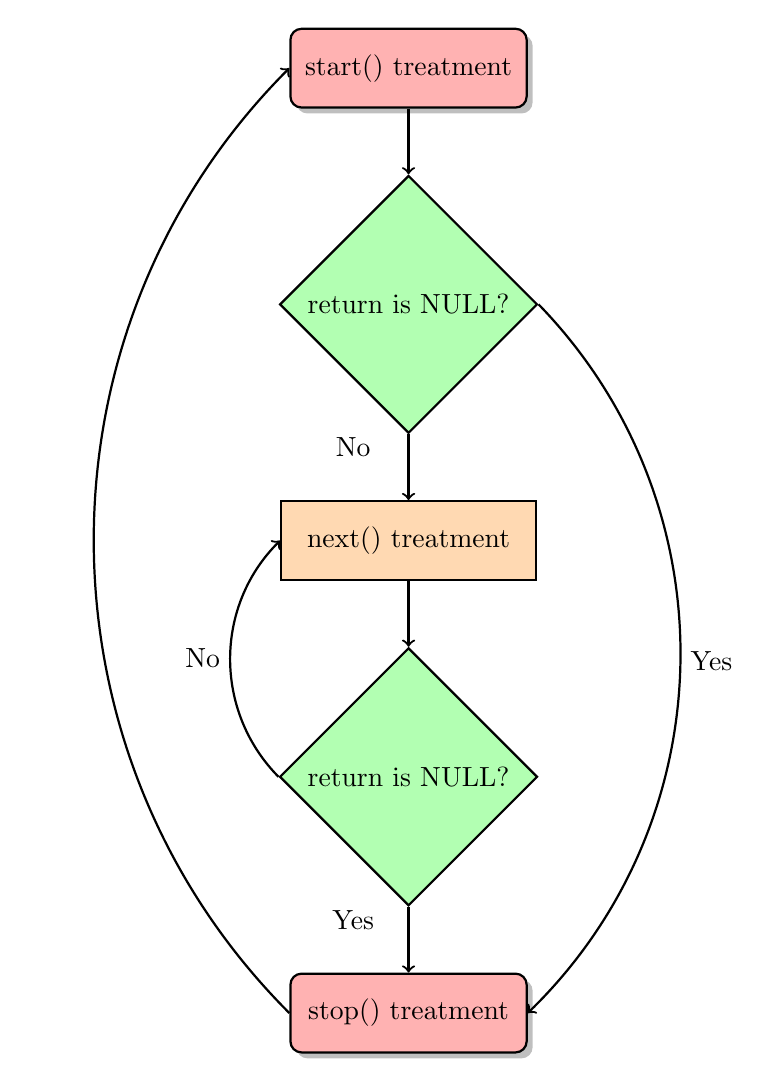
\begin{tikzpicture}[node distance=2cm, thick]
    \node (start) [startstop] {start() treatment};
    \node (branch1) [decision, below of=start, yshift=-1cm] {return is NULL?};
    \node (next) [process, below of=branch1, yshift=-1cm] {next() treatment};
    \node (branch2) [decision, below of=next, yshift=-1cm] {return is NULL?};
    \node (stop) [startstop, below of=branch2, yshift=-1cm] {stop() treatment};

    \draw [->] (start) -- (branch1);
    \draw [->] (branch1.east) to [out=135, in=-135, bend left=45] node [right] {Yes} (stop.east);
    \draw [->] (branch1) -- node[left=2em, anchor=south] {No} (next);
    \draw [->] (next) -- (branch2);
    \draw [->] (branch2.west) to [out=135, in=-135, bend left=45] node [left] {No} (next.west);
    \draw [->] (branch2) -- node[left=2em, anchor=south] {Yes} (stop);
    \draw [->] (stop.west) to [out=135, in=-135] node [left] {} (start.west);
  \end{tikzpicture}
  \caption{How seq\_file works}
  \label{img:seqfile}
\end{figure}

Интерфейс \cpp|seq_file| предоставляет базовые функции для \cpp|proc_ops|, такие как \cpp|seq_read|, \cpp|seq_lseek|и некоторые другие, но ничего для выполнения записи в файл \verb|/proc|.
Хотя вы по-прежнему можете использовать способ из предыдущего примера.

\samplec{examples/procfs4.c}

Если вас интересует дополнительная информация, рекомендую заглянуть на эти страницы:

\begin{itemize}
  \item \url{https://lwn.net/Articles/22355/}
  \item \url{https://kernelnewbies.org/Documents/SeqFileHowTo}
\end{itemize}

Также можете почитать код \src{fs/seq\_file.c} в ядре.

\section{sysfs: взаимодействие с модулем}
\label{sec:sysfs}
\emph{sysfs} позволяет взаимодействовать с работающим ядром из пользовательского пространства, считывая или устанавливая переменные внутри модулей. Это может пригодиться в целях отладки или же в качестве интерфейса для приложений либо скриптов. Каталоги и файлы \emph{sysfs} располагаются в \verb|/sys|.

\begin{codebash}
ls -l /sys
\end{codebash}

Атрибуты для kobjects в этой файловой системе можно экспортировать в форме стандартных файлов. Sysfs перенаправляет файловые операции ввода-вывода в
определенные для этих атрибутов методы, тем самым обеспечивая средства для считывания и записи атрибутов ядра.

Определение атрибута:

\begin{code}
struct attribute {
    char *name;
    struct module *owner;
    umode_t mode;
};

int sysfs_create_file(struct kobject * kobj, const struct attribute * attr);
void sysfs_remove_file(struct kobject * kobj, const struct attribute * attr);
\end{code}

К примеру, модель драйвера определяет \cpp|struct device_attribute| так:

\begin{code}
struct device_attribute {
    struct attribute attr;
    ssize_t (*show)(struct device *dev, struct device_attribute *attr,
                    char *buf);
    ssize_t (*store)(struct device *dev, struct device_attribute *attr,
                    const char *buf, size_t count);
};

int device_create_file(struct device *, const struct device_attribute *);
void device_remove_file(struct device *, const struct device_attribute *);
\end{code}

Чтобы иметь возможность читать и записывать атрибут, при его объявлении необходимо
указать метод \cpp|show()| или \cpp|store()|.
Для распространенных случаев \src{include/linux/sysfs.h} предоставляет удобные макросы (\cpp|__ATTR|, \cpp|__ATTR_RO|, \cpp|__ATTR_WO|, etc.) , упрощая определение атрибутов, а также позволяя сделать код более лаконичным и читаемым.

Вот пример модуля “Hello world”, который включает создание переменной, доступной через sysfs.

\samplec{examples/hello-sysfs.c}

Компиляция и установка модуля:

\begin{codebash}
make
sudo insmod hello-sysfs.ko
\end{codebash}

Убеждаемся в успешности операции:

\begin{codebash}
lsmod | grep hello_sysfs
\end{codebash}

Каково текущее значение \cpp|myvariable| ?

\begin{codebash}
cat /sys/kernel/mymodule/myvariable
\end{codebash}

Установка значения \cpp|myvariable| и проверка, изменилось ли оно:

\begin{codebash}
echo "32" | sudo tee /sys/kernel/mymodule/myvariable
cat /sys/kernel/mymodule/myvariable
\end{codebash}

Наконец, извлечение тестового модуля:

\begin{codebash}
sudo rmmod hello_sysfs
\end{codebash}

В случае выше мы используем для создания каталога в sysfs и взаимодействия с его атрибутами простой \cpp|kobject| Начиная с Linux v2.6.0, структура \cpp|kobject| постепенно обретала свой нынешний облик.
Изначально она подразумевалась как простой способ унификации кода ядра, управляющего объектами с подсчетом ссылок. Однако спустя некоторое время ее
назначение расширилось, и теперь она связывает большую часть модели устройства и ее интерфейса sysfs.
Подробнее о kobject и sysfs читайте в \src{Documentation/driver-api/driver-model/driver.rst} and \url{https://lwn.net/Articles/51437/}.

\section{Взаимодействие с файлами устройств}
\label{sec:device_files}
Файлы устройств представляют физические устройства. Большинство таких устройств используются для вывода и ввода, а значит необходим некий механизм, который бы позволил их находящимся в ядре драйверам получать вывод от процессов для его перенаправления самим устройствам. Для этого файл открывается, и в него производится запись, в точности аналогично стандартной операции записи в файл. В примере ниже это реализовано с помощью \cpp|device_write|.

Но этого не всегда оказывается достаточно. Представьте, что у вас к последовательному порту подключен модем (даже если модем внутренний, эта схема с точки зрения процессора все равно реализуется как модем, подключенный к последовательному порту, так что воображение особо напрягать не нужно).

Естественным решением здесь будет использовать файл устройства как для записи на модем (к примеру, команд или данных для отправки), так и для чтения с него (например, ответов на команды или полученных данных). Тем не менее остается вопрос о том, что же делать, когда нужно взаимодействовать с самим последовательным портом, например, для настройки скорости отправки/получения данных.

В Unix ответом будет использовать специальную функцию \cpp|ioctl| ((сокращенно от Input
Output ConTroL). Каждое устройство может иметь собственные команды \cpp|ioctl| cреализующие чтение (для отправки информации от процесса ядру), запись (для
возвращения информации процессу), и то и другое, либо ни одно из этих действий.
Имейте ввиду, что в \cpp|ioctl| роли чтения и записи снова реверсируются, то есть при чтении происходит отправка информации ядру, а при записи ее получение от ядра. Вызывается функция ioctl с тремя параметрами: дескриптором соответствующего файла устройства, номером ioctl и параметром, имеющим тип long, чтобы можно было использовать приведение, позволяющее с его помощью передавать почти все, что захочется.
Таким способом не удастся передать структуру, но можно будет передать указатель на нее. Вот пример:

\samplec{examples/ioctl.c}

Вы можете заметить в функции \cpp|test_ioctl_ioctl()| аргумент \cpp|cmd|.
Это номер ioctl.
Он кодирует старший (major) номер устройства, тип ioctl, команду и тип параметра. Обычно этот номер создается вызовом макроса (\cpp|_IO|, \cpp|_IOR|, \cpp|_IOW| или \cpp|_IOWR| — в зависимости от типа) в заголовочном файле.
Этот заголовочный файл должен быть включен и в программы, которые будут использовать ioctl (чтобы они могли генерировать подходящие ioctl), и в модуль ядра (чтобы он мог эту функцию понимать). В примере ниже заголовочным файлом является \verb|chardev.h|, а использующей его
программой \verb|userspace_ioctl.c|.

Если вы хотите использовать ioctl в собственных модулях, то лучше будет получить для нее официальное назначение. Тогда, если у вас каким-то образом окажется чужая ioctl, то сразу станет понятно, что что-то не так.
Более подробную информацию можно получить в дереве исходного кода ядра на странице \src{Documentation/userspace-api/ioctl/ioctl-number.rst}.

Кроме того, необходимо иметь ввиду, что конкурентное обращение к ресурсам приведет к
состоянию гонки. Решением будет использовать атомарную инструкцию сравнения с
обменом (CAS), которая упоминалась в \ref{sec:chardev_c}, чтобы организовать индивидуальный доступ.

\samplec{examples/chardev2.c}

\samplec{examples/chardev.h}

\samplec{examples/other/userspace_ioctl.c}

\section{Системные вызовы}
\label{sec:syscall}
До этого момента мы просто использовали отлаженные механизмы ядра для регистрации файлов \verb|/proc| и обработчиков устройств. И это отличное решение, когда вы хотите сделать нечто стандартное, что предполагали программисты ядра, например написать драйвер устройства. Но как быть, если вы планируете сделать что-то необычное, каким-то образом изменить поведение системы? Здесь вам придется действовать полностью самостоятельно.

И если вы пойдете рисковым путем, не задействовав виртуальную машину, то программирование ядра уже может стать весьма опасным занятием. В процессе
написания примера, который вы увидите ниже, я убил системный вызов \cpp|open()| и в итоге не смог открывать какие-либо файлы, запускать программы и даже выключить систему. Пришлось перезапускать виртуальную машину. Никакие важные файлы не пострадали, но если бы я делал то же самое в реальной критически важной системе, то такой исход оказался бы вполне вероятен. Чтобы оградить себя от возможной потери каких-либо файлов, даже в рамках тестовой среды, рекомендую до выполнения \sh|insmod| и \sh|rmmod| выполнять \sh|sync|.

Забудьте о файлах \verb|/proc| забудьте о файлах устройств – это лишь мелкие детали в необъятном пространстве вселенной. Реальным механизмом в контексте взаимодействия с ядром, тем, который используют все процессы, являются системные вызовы. Когда процесс запрашивает у ядра операцию (например, открытие файла, разветвление на новый процесс или выделение дополнительной памяти), используется именно этот механизм.
Если вы хотите изменить поведение ядра, то вмешательство производится как раз в него.
Кстати, посмотреть, какие системные вызовы использует программа, можно так: \sh|strace <arguments>|.

Как правило, процесс не должен иметь возможности обращаться к ядру, то есть он не может обращаться к его памяти и вызывать его функции. Это обусловлено аппаратной спецификой ЦПУ (именно поэтому мы говорим «защищенный режим» или «защита страниц»).
И системные вызовы являются в этом общем правиле исключением. Технически это происходит так – процесс заполняет регистр нужными значениями, после чего вызывает особую инструкцию, которая переключается на ранее определенную область ядра (естественно, эта область доступна пользовательским процессам только для чтения, но не для записи). В случае процессоров Intel это происходит посредством прерывания 0х80.

Аппаратное обеспечение знает, что при переходе в эту область вы выходите из ограниченного пользовательского режима, начиная действовать уже в юрисдикции ядра, в связи с чем для вас открываются все двери.

% FIXME: recent kernel changes the system call entries
Область ядра, в которую может перескочить процесс, называется \verb|system_call|.
Процедура в этой области проверяет номер системного вызова, сообщая ядру о том,
какое действие процесс запросил. Затем она просматривает таблицу системных вызовов (\cpp|sys_call_table|) в поиске адреса нужной функции ядра. Далее она эту функцию вызывает, и после того, как та возвращает результат, выполняет ряд системных проверок и делает возврат процессу (или к другому процессу, если время изначального истекло).

Прописан весь этот код в файле \verb|arch/$(architecture)/kernel/entry.S| после строки \cpp|ENTRY(system_call)|.

Итак, если мы хотим изменить способ работы определенного системного вызова, то нам нужно написать собственную функцию для его реализации (обычно для этого добавляется собственный код, после чего вызывается оригинальная функция), а затем перевести указатель в \cpp|sys_call_table| на нашу новую функцию. Поскольку позднее эта функция может быть удалена, важно, чтобы \cpp|cleanup_module| восстанавливала таблицу в исходное состояние.

Для изменения содержимого \cpp|sys_call_table|, необходимо взять во внимание регистр управления. Это регистр процессора, который изменяет или управляет его общим функционированием. В архитектуре x86 у регистра \verb|cr0| rесть различные флаги управления, которые изменяют основные операции процессора. Среди них есть флаг \verb|WP|, который отвечает за защиту от записи. Если он установлен, процессор запрещает выполнение записи в разделы только для чтения. Следовательно, прежде чем изменять \cpp|sys_call_table| нам нужно этот флаг отключить.
Начиная с Linux v5.3, функцию \cpp|write_cr0| использовать нельзя из-за чувствительных бит \verb|cr0|, представляющих угрозу безопасности. С их помощью атакующий может производить запись в регистры управления, отключая защиты ЦПУ, например защиту от записи. В итоге для обхода этого ограничения необходимо предоставить собственную подпрограмму ассемблера.

Однако символ \cpp|sys_call_table| с целью предотвращения подобного трюка является неэкспортируемым. Но у нас все же есть пара способов для его получения, а именно ручной поиск символов и \cpp|kallsyms_lookup_name|. Здесь мы рассмотрим использование обоих, в зависимости от версии ядра.

В ядре используется механизм Control-Flow Integrity (CFI), предназначенный для предотвращения возможного перенаправления исполнения кода атакующим. Он
позволяет гарантировать направление косвенных вызовов к ожидаемым адресам, а также неизменность возвращаемых адресов. Начиная с Linux v5.7, в ядре пропатчили ряд методов Control-Flow Enforcement (CET) для архитектуры x86, и некоторые конфигурации GCC, например GCC 9 и 10 версии, будут идти с CET (опция \verb|-fcf-protection|) по умолчанию. Использование этого GCC для компиляции ядра при отключенном Retpoline может привести к активации в ядре функционала CET.

Проверить, включена ли опция \verb|-fcf-protection|, можно следующей командой:
\begin{verbatim}
$ gcc -v -Q -O2 --help=target | grep protection
Using built-in specs.
COLLECT_GCC=gcc
COLLECT_LTO_WRAPPER=/usr/lib/gcc/x86_64-linux-gnu/9/lto-wrapper
...
gcc version 9.3.0 (Ubuntu 9.3.0-17ubuntu1~20.04)
COLLECT_GCC_OPTIONS='-v' '-Q' '-O2' '--help=target' '-mtune=generic' '-march=x86-64'
 /usr/lib/gcc/x86_64-linux-gnu/9/cc1 -v ... -fcf-protection ...
 GNU C17 (Ubuntu 9.3.0-17ubuntu1~20.04) version 9.3.0 (x86_64-linux-gnu)
...
\end{verbatim}
Но CET не должен быть включен в ядре, поскольку это может нарушить работу Kprobes и bpf. По этой причине, начиная с v5.11, данный функционал был отключен. Поэтому, чтобы у нас гарантированно работал ручной поиск символов, мы используем версии ядра до v5.4.

К сожалению, начиная с Linux v5.7, \cpp|kallsyms_lookup_name| также не экспортируется, и получить адрес этой функции можно лишь обходным путем. Если включена опция If \cpp|CONFIG_KPROBES|, можно извлечь этот адрес, используя Kprobes для динамического проникновения в определенную подпрограмму ядра. Kprobe вставляет точку останова на входе функции, заменяя первые байты просматриваемой инструкции. Когда ЦПУ достигает этой точки останова, регистры сохраняются, и управление переходит Kprobes. Он передает адреса сохраненных регистров и структуры Kprobe заданному нами обработчику, после чего его запускает. Kprobes можно зарегистрировать по имени символа или адресу. При использовании имени символа адрес будет обрабатываться ядром.

В противном случае указать адрес \cpp|sys_call_table| из \verb|/proc/kallsyms| и \verb|/boot/System.map| в параметре \cpp|sym|.
Вот пример использования \verb|/proc/kallsyms|:
\begin{verbatim}
$ sudo grep sys_call_table /proc/kallsyms
ffffffff82000280 R x32_sys_call_table
ffffffff820013a0 R sys_call_table
ffffffff820023e0 R ia32_sys_call_table
$ sudo insmod syscall-steal.ko sym=0xffffffff820013a0
\end{verbatim}

При использовании адреса из \verb|/boot/System.map| будьте внимательны к \verb|KASLR| (рандомизация адресного пространства ядра). Этот механизм может рандомизировать адреса кода ядра и данных при каждой загрузке. К примеру, статический адрес, указанный в \verb|/boot/System.map|, сдвигается на некоторое случайное значение.
Задача \verb|KASLR| – защищать пространство ядра от атак. В случае отсутствия этого механизма атакующему было бы проще отыскать фиксированный целевой адрес, после чего с помощью возвратно-ориентированного программирования вставить вредоносный код для выполнения или получения нужных данных по фиктивному указателю.
Without \verb|KASLR|, the attacker may find the target address in the fixed address easily.
Then the attacker can use return-oriented programming to insert some malicious codes to execute or receive the target data by a tampered pointer.
\verb|KASLR| противостоит подобным атакам, не позволяя атакующему прямиком узнать целевой адрес. Хотя метод подбора здесь все еще может сработать. Если адрес символа в \verb|/proc/kallsyms| отличается от адреса в \verb|/boot/System.map| ядро активирует \verb|KASLR|.

\begin{verbatim}
$ grep GRUB_CMDLINE_LINUX_DEFAULT /etc/default/grub
GRUB_CMDLINE_LINUX_DEFAULT="quiet splash"
$ sudo grep sys_call_table /boot/System.map-$(uname -r)
ffffffff82000300 R sys_call_table
$ sudo grep sys_call_table /proc/kallsyms
ffffffff820013a0 R sys_call_table
# Reboot
$ sudo grep sys_call_table /boot/System.map-$(uname -r)
ffffffff82000300 R sys_call_table
$ sudo grep sys_call_table /proc/kallsyms 
ffffffff86400300 R sys_call_table
\end{verbatim}

Если \verb|KASLR| iактивна, то после каждой перезагрузки необходимо уделять внимание адресу из \verb|/proc/kallsyms|.
Поэтому для использования адреса из \verb|/boot/System.map| нужно будет убедиться, что \verb|KASLR| отключена.
Отключить его можно, добавив при очередной загрузке параметр \verb|nokaslr|:

\begin{verbatim}
$ grep GRUB_CMDLINE_LINUX_DEFAULT /etc/default/grub
GRUB_CMDLINE_LINUX_DEFAULT="quiet splash"
$ sudo perl -i -pe 'm/quiet/ and s//quiet nokaslr/' /etc/default/grub
$ grep quiet /etc/default/grub
GRUB_CMDLINE_LINUX_DEFAULT="quiet nokaslr splash"
$ sudo update-grub
\end{verbatim}

Дополнительно по этой теме читайте:

\begin{itemize}
 \item \href{https://lwn.net/Articles/804849/}{Cook: Security things in Linux v5.3}
 \item \href{https://lwn.net/Articles/12211/}{Unexporting the system call table}
 \item \href{https://lwn.net/Articles/810077/}{Control-flow integrity for the kernel}
 \item \href{https://lwn.net/Articles/813350/}{Unexporting kallsyms\_lookup\_name()}
 \item \href{https://www.kernel.org/doc/Documentation/kprobes.txt}{Kernel Probes (Kprobes)}
 \item \href{https://lwn.net/Articles/569635/}{Kernel address space layout randomization}
\end{itemize}

Приведенный здесь исходный код является примером подобного модуля ядра. Мы хотим
реализовать «слежку» за определенным пользователем и выводить \cpp|pr_info()| сообщение при каждом открытии им файла.
С этой целью мы заменяем системный вызов собственной функцией\cpp|our_sys_openat|.
 Эта функция проверяет uid текущего процесса, и если оно совпадает с uid, за которым мы следим, вызывает\cpp|pr_info()| для
отображения имени открываемого файла. Затем она в любом случае вызывает оригинальную функцию \cpp|openat()| с теми же параметрами, чтобы уже реально открыть файл.

Функция \cpp|init_module| заменяет нужную запись в \cpp|sys_call_table| и сохраняет оригинальный указатель в переменной.
В последствии функция \cpp|cleanup_module| использует эту переменную для восстановления исходного состояния таблицы. Это опасный подход, поскольку есть
вероятность, что два модуля изменят один и тот же системный вызов.
Представьте, что у нас есть два модуля, A и B. У А системным вызовом для открытия файла будет \cpp|A_openat|, а у В им будет \cpp|B_openat|.
Теперь, при внедрении А в ядро соответствующий системный вызов будет заменен на \cpp|A_openat|, который по завершению вызовет \cpp|sys_openat|. Далее в ядро внедряется В, заменяя системный вызов А на \cpp|B_openat|, который по завершению вызовет тот самый, \cpp|A_openat|, являющийся для него ригинальным.

Теперь, если первым будет удален В, то все нормально – он просто восстановит системный вызов на \cpp|A_openat|, который вызывает оригинал. Но вот если сначала удалить А, а затем В, то в системе произойдет сбой. Удаление А приведет к восстановлению исходного системного вызова, \cpp|sys_openat|, исключив из процесса B.

Затем, когда будет удаляться В, он постарается восстановить системный вызов на тот, который считает исходным, то есть \cpp|A_openat|, но его в памяти уже не окажется.

На первый взгляд эту проблему можно разрешить, проверив, совпадает ли системный вызов с нашей функцией открытия – если да, то просто его не менять (чтобы В не трогал системный вызов при удалении). Но это создаст еще большую проблему.

При удалении А увидит, что системный вызов был заменен на \cpp|B_openat| и больше не указывает на \cpp|A_openat|, а значит не станет восстанавливать его на \cpp|sys_openat|, пока не будет удален из памяти.
К сожалению, в итоге В по-прежнему будет пытаться вызвать \cpp|A_openat|, которого больше нет, так что даже без удаления В система все равно даст сбой.

Заметьте, что все описанные проблемы делают перехват системных вызовов нецелесообразным для использования в продакшн-среде. И для того, чтобы оградить
людей от совершения потенциально вредных действий, \cpp|sys_call_table| больше не экспортируется.

То есть, если вы хотите сделать что-то большее, нежели просто выполнить этот пример, то вам потребуется пропатчить ядро, чтобы вернуть поддержку экспорта \cpp|sys_call_table|.

\samplec{examples/syscall-steal.c}

\section{Блокировка процессов и потоков}
\label{sec:blocking_process_thread}
\subsection{Ожидание}
\label{sec:sleep}
Что вы делаете, когда вас просят сделать что-то, чем пока вы заняться не можете? Как обычный человек, которого просит другой такой же человек, вы на это можете сказать лишь: «Я пока занят. Не мешай». Но если вы являетесь ядром, а обратился к вам процесс, то у вас есть другой вариант.
Вы можете поставить этот процесс в режим ожидания (sleep), пока не появится возможность его обслужить. По факту ядро постоянно отправляет процессы в ожидание и пробуждает их. Именно так реализовано одновременное выполнение множества процессов на одном ЦПУ.

И текущий модуль ядра является примером этого. Файл (с именем \verb|/proc/sleep|) одновременно может быть открыт лишь одним процессом. Если он уже открыт, модуль вызывает \cpp|wait_event_interruptible|.
Самый простой способ сохранять файл открытым – это использовать команду:

\begin{codebash}
tail -f
\end{codebash}

Эта функция изменяет статус задачи (задача – это структура данных ядра, содержащая информацию о процессе и системном вызове, в котором он находится, если таковой присутствует) на \cpp|TASK_INTERRUPTIBLE|. Это означает, что выполнение задачи будет отложено до момента ее пробуждения, а пока она добавляется в WaitQ, то есть очередь задач, ожидающих возможности получить доступ к файлу. Затем эта функция вызывает планировщик для переключения контекста на другой процесс, которому нужен ЦПУ.

Когда процесс закончил работу с файлом, он его закрывает, и вызывается \cpp|module_close|. Эта функция пробуждает все процессы в очереди (не существует механизма для пробуждения их по одиночке), после чего делает возврат, и процесс, закрывший файл, может продолжать свое выполнение. Далее в свое время планировщик решает, что этот процесс уже достаточно поработал, и передает управление ЦПУ другому процессу из очереди. Свое выполнение этот процесс начинает с момента, следующего сразу за вызовом \cpp|wait_event_interruptible|.

Это означает, что процесс все еще находится в режиме ядра – по имеющейся у него информации, он отправил системный вызов open(), который возврат еще не сделал. Процессу не известно, что большую часть времени между моментом отправки этого вызова и его возвратом ЦПУ использовался кем-то еще.

После этого он может установить глобальную переменную, указывающую всем другим процессам, что файл пока открыт, и продолжить выполнение. Когда другие процессы будут получать долю внимания ЦПУ, они будут видеть эту установленную переменную и возвращаться в режим ожидания.

Итак, мы используем \sh|tail -f|, чтобы фоново удерживать файл в открытом состоянии при попытке получить к нему доступ другим процессом (также в фоновом режиме, чтобы не пришлось переключаться на другой VT). Как только первый фоновый процесс завершится командой kill \%1, пробудится второй, который получит доступ к файлу, а затем также завершится.

При этом \cpp|module_close| не единственный, кто имеет право на пробуждение процессов,
ожидающих доступа к файлу. Помимо этого, они могут пробуждаться сигналом \emph{Ctrl +c} (\textbf{SIGINT}). Причина тому в использованной нами функции \cpp|wait_event_interruptible|.
Можно было задействовать \cpp|wait_event| но это бы сильно разозлило пользователей, чьи нажатия \emph{Ctrl+c} тогда бы игнорировались.
В этом случае нам нужно сразу же возвращать \cpp|-EINTR| Это необходимо, чтобы пользователи могли, например, завершить процесс до получения им доступа к файлу. Нужно помнить и еще кое-что. Иногда процессы не хотят спать, они хотят незамедлительно получить либо желаемое, либо ответ, что это действие выполнить нельзя. Подобные процессы используют при открытии файла флаг cpp|O_NONBLOCK|

На это ядро должно возвращать код ошибки \cpp|-EAGAIN| от операций, которые в противном
случае должны были заблокироваться, к примеру, при открытии файла, как в нашем примере. Для открытия файла с \cpp|O_NONBLOCK| можно использовать программу, расположенную в каталоге \sh|cat_nonblock| \verb|examples/other|.

\begin{verbatim}
$ sudo insmod sleep.ko
$ cat_nonblock /proc/sleep
Last input:
$ tail -f /proc/sleep &
Last input:
Last input:
Last input:
Last input:
Last input:
Last input:
Last input:
tail: /proc/sleep: file truncated
[1] 6540
$ cat_nonblock /proc/sleep
Open would block
$ kill %1
[1]+  Terminated              tail -f /proc/sleep
$ cat_nonblock /proc/sleep
Last input:
$
\end{verbatim}

\samplec{examples/sleep.c}

\samplec{examples/other/cat_nonblock.c}

\subsection{Завершение потоков}
\label{sec:completion}
Иногда в модуле, имеющем несколько потоков, одно действие должно совершиться перед другим. И вместо использования команд \sh|/bin/sleep|, ядро реализует это другим способом, поддерживающим таймауты или прерывания.В примере ниже стартуют два потока, но один должен сработать раньше.

Completions as code synchronization mechanism have three main parts, initialization of struct completion synchronization object, the waiting or barrier part through \cpp|wait_for_completion()|, and the signalling side through a call to \cpp|complete()|.

In the subsequent example, two threads are initiated: crank and flywheel. 
It is imperative that the crank thread starts before the flywheel thread. 
A completion state is established for each of these threads, with a distinct completion defined for both the crank and flywheel threads.
At the exit point of each thread the respective completion state is updated, and \cpp|wait_for_completion| is used by the flywheel thread to ensure that it does not begin prematurely.
The crank thread uses the \cpp|complete_all()| function to update the completion, which lets the flywheel thread continue.

Так что, хоть \cpp|flywheel_thread| и стартует первым, загрузив модуль и выполнив \sh|dmesg|, вы должны заметить, что сначала всегда происходит поворот рычага (crank), потому что поток маховика (flywheel) ожидает его завершения.

У функции \cpp|wait_for_completion| есть и другие вариации, которые включают таймауты и прерывания, но этого базового механизма вполне достаточно для множества типичных ситуаций без добавления излишней сложности.

\samplec{examples/completions.c}

\section{Избегание коллизий и взаимных блокировок}
\label{sec:synchronization}
Если процессы, выполняющиеся на разных ядрах или в разных потоках, попытаются обратиться к одной и той же области памяти, то вполне могут случиться странности, либо система просто заблокируется.
Для избежания этого в ядре существуют специальные функции взаимного исключения (мьютексы).
Они показывают, «занят» или «свободен» в данный момент фрагмент кода, исключая тем самым одновременные попытки его выполнения.
\subsection{Mutex}
\label{sec:mutex}
Используются мьютексы ядра аналогично тому, как они развертываются в пользовательской среде.
И в большинстве случаев для избежания коллизий этого вполне может оказаться достаточно.

\samplec{examples/example_mutex.c}

\subsection{Spinlocks}
\label{sec:spinlock}
Спин-блокировки, или спинлоки, блокируют ЦПУ, на котором выполняется код, занимая 100\% его ресурсов. В связи с этим механизм спинлоков желательно использовать только для кода, на выполнение которого требуется не более нескольких миллисекунд, чтобы с позиции пользователя не вызвать заметного замедления работы.

Примером в данном случае является ситуация \verb|"irq safe"|, когда прерывания, происходящие во время блокировки, не забываются, а повторно активируются при ее снятии, используя переменную \cpp|flags| для сохранения своего состояния.

\samplec{examples/example_spinlock.c}

\subsection{Блокировки для чтения и записи}
\label{sec:rwlock}
Блокировки для выполнения чтения и записи – это специализированные спинлоки, позволяющие эксклюзивно считывать или производить запись.
Подобно предыдущему примеру, код ниже показывает ситуацию "irq safe", когда в случае активации аппаратными прерываниями других функций, которое также могут выполнять нужные вам чтение/запись, эти функции не нарушат текущую логику выполнения.
Как и прежде, будет правильным решением, устанавливать подобную блокировку для максимально коротких задач, чтобы они не подвешивали систему и не вызывали
недовольство пользователей относительно тирании вашего модуля.

\samplec{examples/example_rwlock.c}

Конечно же, если вы уверены, что аппаратные прерывания не активируют никакие функции, которые могли бы нарушить логику, то можете использовать более простые \cpp|read_lock(&myrwlock)| and \cpp|read_unlock(&myrwlock)| либо соответствующие функции записи.
\subsection{Атомарные операции}
\label{sec:atomics}
Если вы выполняете простую арифметику: сложение, вычитание или побитовые операции, тогда многоядерный и гиперпоточный мир может предложить еще один способ, как не позволить другим компонентам системы вмешаться в ваше действо. С помощью атомарных операций вы можете обеспечить, чтобы ваше сложение, вычитание или инвертирование битов произошли успешно и не были перезаписаны какими-либо сторонними процессами. Вот пример:

\samplec{examples/example_atomic.c}

До того, как в стандарте С11 появились встроенные атомарные типы, ядро уже предоставляло небольшой их набор, которым можно было воспользоваться с помощью
хитрого архитектурно-зависимого кода.

Реализация же атомарных типов в С11 позволяет ядру отказаться от этих специфичных команд, сделав его код более внятным для людей, которые данный стандарт понимают. Но есть здесь и кое-какие проблемы, например модель памяти ядра не соответствует модели, формируемой атомарными операциями в С11. Подробнее эта тема раскрыта в следующих ресурсах:
\begin{itemize}
 \item \href{https://www.kernel.org/doc/Documentation/atomic_t.txt}{kernel documentation of atomic types}
 \item \href{https://lwn.net/Articles/691128/}{Time to move to C11 atomics?}
 \item \href{https://lwn.net/Articles/698315/}{Atomic usage patterns in the kernel}
\end{itemize}

% FIXME: we should rewrite this section
\section{Замена макроса Prints}
\label{sec:print_macros}
\subsection{Замена}
% FIXME: cross-reference
В разделе \ref{sec:preparation} я говорил, что программировать модули ядра через X Window System не желательно. Это верно относительно именно разработки модулей, но при фактическом использовании нам нужна возможность отправлять сообщения на любой tty, с которого поступила команда на загрузку модуля.

Аббревиатура tty означает телетайп, устройство, которое в своем изначальном виде представляло совмещенную с принтером клавиатуру, используемую для взаимодействия с системой Unix.

В современном же представлении телетайп является абстракцией текстового потока, используемой программой Unix, будь то физический терминал, xterm на X-сервере, сетевое подключение через ssh или нечто аналогичное.

Реализуется это с помощью ``current'', указателя на выполняемую в данный момент задачу, позволяющего получить tty-структуру этой задачи. Затем эта структура просматривается в поиске указателя на строковую функцию write, которая используется для записи строки в данный tty.

\samplec{examples/print_string.c}

\subsection{Мигание светодиодами клавиатуры}
\label{sec:flash_kb_led}
В определенных условиях вы можете предпочесть более простой и непосредственный способ связи с внешним миром. Решением в таком случае может стать мигание
светодиодами клавиатуры. Это прямой способ привлечь внимание или продемонстрировать некое состояние. Светодиоды есть у любой клавиатуры, они всегда
на виду, не требуют настройки и очень просты в использовании, если сравнивать с записью в tty или файл.

В v4.14 и v.4.15 в API таймера произошел ряд изменений, нацеленных на повышение безопасности памяти. Переполнение буфера в области структуры \cpp|timer_list| может привести к перезаписи полей \cpp|function| и \cpp|data|, предоставив атакующему возможность с
помощью возвратно-объектного программирование вызывать произвольные функции в ядре.

Кроме того, прототип функции обратного вызова, содержащий аргумент \cpp|unsigned long| полностью исключит возможность проверки типов. Плюс такой прототип может помешать защитить косвенные переходы и вызовы (forward-edge) с помощью сохранения целостности потока управления (CFI).

Поэтому лучше использовать уникальный прототип, чтобы отделиться от кластера, который получает аргумент \cpp|unsigned long|. В обратный вызов таймера необходимо передавать не аргумент \cpp|unsigned long|, а указатель на структуру \cpp|timer_list|.

Тогда он объединит всю необходимую ему информацию, включая структуру \cpp|timer_list| в более обширную структуру и сможет использовать вместо значения \cpp|unsigned long| макрос \cpp|container_of|.

Более развернуто эта тема описана в статье: \href{https://lwn.net/Articles/735887/}{Improving the kernel timers API}.

До Linux v4.14 инициализация таймеров производилась с помощью \cpp|setup_timer|, а структура \cpp|timer_list| выглядела так:
\begin{code}
struct timer_list {
    unsigned long expires;
    void (*function)(unsigned long);
    unsigned long data;
    u32 flags;
    /* ... */
};

void setup_timer(struct timer_list *timer, void (*callback)(unsigned long),
                 unsigned long data);
\end{code}

В Linux v4.14 появилась \cpp|timer_setup|, и ядро постепенно перестроилось с \cpp|setup_timer| на \cpp|timer_setup|.
Одна из причин изменения API заключалась в потребности сосуществования с интерфейсом старых версий. Более того, по началу \cpp|timer_setup| реализовывалась через \cpp|setup_timer|.

\begin{code}
void timer_setup(struct timer_list *timer,
                 void (*callback)(struct timer_list *), unsigned int flags);
\end{code}

Позднее в v4.15 \cpp|setup_timer| удалили, что также отразилось на облике структуры \cpp|timer_list|.
\begin{code}
struct timer_list {
    unsigned long expires;
    void (*function)(struct timer_list *);
    u32 flags;
    /* ... */
};
\end{code}

Приведенный ниже код демонстрирует минимальный модуль ядра, который после загрузки начинает мигать светодиодами до тех пор, пока не будет выгружен.

\samplec{examples/kbleds.c}

Если ни один из приведенных в этой главе примеров не подходит под ваши отладочные нужды, то наверняка есть другие решения. Не задумывались, для чего может быть полезна \cpp|CONFIG_LL_DEBUG| из \sh|make menuconfig|?
В случае ее активации вы получаете низкоуровневый доступ к последовательному порту. И хотя это может не показаться особо полезным, такой прием позволяет пропатчить \src{kernel/printk.c} или любой другой важный системный вызов для печати символов ASCII, делая возможным отслеживание практически всех действий кода на последовательном порту.

Если вы займетесь портированием ядра на новую, ранее неподдерживаемую архитектуру, то реализация этого решения должна идти одной из первых. Также можно рассмотреть вариант логирования через netconsole.

Несмотря на множество рассмотренных здесь отладочных приемов, кое-что нужно иметь ввиду. Отладка практически всегда оказывается интрузивной процедурой. Добавление отладочного кода может привести к тому, что ошибка, на первый взгляд, исчезнет. Поэтому такой код нужно минимизировать и следить, чтобы он не попал в продакшн-код.

\section{GPIO}
\label{sec:gpio}
\subsection{GPIO}
\label{sec:gpio_introduction}
General Purpose Input/Output (GPIO) appears on the development board as pins.
It acts as a bridge for communication between the development board and external devices.
You can think of it like a switch: users can turn it on or off (Input), and the development board can also turn it on or off (Output).

To implement a GPIO device driver, you use the \cpp|gpio_request()| function to enable a specific GPIO pin.
After successfully enabling it, you can check that the pin is being used by looking at /sys/kernel/debug/gpio.

\begin{codebash}
cat /sys/kernel/debug/gpio
\end{codebash}

There are other ways to register GPIOs.
For example, you can use \cpp|gpio_request_one()| to register a GPIO while setting its direction (input or output) and initial state at the same time.
You can also use \cpp|gpio_request_array()| to register multiple GPIOs at once. However, note that \cpp|gpio_request_array()| has been removed since Linux v6.10+.

When using GPIO, you must set it as either output with \cpp|gpio_direction_output()| or input with \cpp|gpio_direction_input()|.

\begin{itemize}
  \item when the GPIO is set as output, you can use \cpp|gpio_set_value()| to choose to set it to high voltage or low voltage.
  \item when the GPIO is set as input, you can use \cpp|gpio_get_value()| to read whether the voltage is high or low.
\end{itemize}

\subsection{Control the LED's on/off state}
\label{sec:gpio_led}
In Section \ref{sec:device_files}, we learned how to communicate with device files.
Therefore, we will further use device files to control the LED on and off.

In the implementation, a pull-down resistor is used.
The anode of the LED is connected to GPIO4, and the cathode is connected to GND.
For more details about the Raspberry Pi pin assignments, refer to \href{https://pinout.xyz/}{Raspberry Pi Pinout}.
The materials used include a Raspberry Pi 5, an LED, jumper wires, and a 220$\Omega$ resistor.

\samplec{examples/led.c}

Make and install the module:
\begin{codebash}
make
sudo insmod led.ko
\end{codebash}

Switch on the LED:
\begin{codebash}
echo "1" | sudo tee /dev/gpio_led
\end{codebash}

Switch off the LED:
\begin{codebash}
echo "0" | sudo tee /dev/gpio_led
\end{codebash}

Finally, remove the module:
\begin{codebash}
sudo rmmod led
\end{codebash}

\section{Планирование задач}
\label{sec:scheduling_tasks}
Есть два основных способа выполнения задач: тасклеты и очереди заданий. Тасклеты – это быстрый и простой способ планирования выполнения одной функции, например, при ее активации прерыванием.
А вот очереди заданий хоть и более сложны, но зато лучше подходят для выполнения последовательностей задач.

\subsection{Тасклеты}
\label{sec:tasklet}
Ниже показан пример модуля тасклета. Функция \cpp|tasklet_fn| выполняется несколько секунд. При этом выполнение функции \cpp|example_tasklet_init| может продолжаться до точки выхода, что будет зависеть от того, была ли она прервана \textbf{softirq}.

\samplec{examples/example_tasklet.c}

После загрузки этого примера \sh|dmesg| должна отобразить следующее:

\begin{verbatim}
tasklet example init
Example tasklet starts
Example tasklet init continues...
Example tasklet ends
\end{verbatim}

И хотя использовать тасклеты легко, они имеют несколько недостатков, и в среде разработчиков обсуждается их возможное исключение из ядра. Обратный вызов тасклета выполняется в атомарном контексте внутри программного прерывания, то есть он не может входить в режим ожидания или получать доступ к данным пользовательского пространства, в результате чего в обработчике тасклетов не получится выполнить всю работу. Кроме того, ядро разрешает одновременно выполнять только один экземпляр любого конкретного тасклета. При этом несколько разных могут выполняться параллельно.

В последних версиях ядра появилась возможность заменить тасклеты очередями заданий, таймерами или прерываниями, выносимыми в отдельные потоки (threaded
interrupts). Пока удаление тасклетов продолжает оставаться долгосрочной целью, в своем текущем виде ядро содержит более сотни случаев их использования. Сейчас разработчики продолжают вносить изменения в API, и для совместимости существует макрос \cpp|DECLARE_TASKLET_OLD|.

Подробнее читайте на странице \url{https://lwn.net/Articles/830964/}.

\subsection{Очереди заданий}
\label{sec:workqueue}
Добавлять задачи в планировщик можно через очередь заданий. Для выполнения прописанных в этой очереди задач ядро использует Completely Fair Scheduler (CFS).

\samplec{examples/sched.c}

\section{Обработка прерываний}
\label{sec:interrupt_handler}
\subsection{Interrupt Handlers}
\label{sec:irq}
Во всех главах (за исключением предыдущей), мы реализовывали в ядре лишь ответы на
запросы процессов, для чего-либо работали с особым файлом, либо отправляли \cpp|ioctl()|или системный вызов. Но работа ядра состоит не только в реагировании на запросы процессов. Ещё одной его немаловажной ответственностью является взаимодействие с подключённым к машине оборудованием.

Существует два типа взаимодействий между ЦПУ и остальным оборудованием компьютера. Первый – это когда ЦПУ отдаёт ему распоряжения. Распоряжение
подразумевает, что оборудование должно сообщить что-либо процессору. Второй, называемый прерываниями, уже гораздо сложнее в реализации, поскольку
обрабатывается, когда это нужно оборудованию, а не процессору. Как правило, аппаратные средства оснащены очень небольшим объёмом оперативной памяти, и если своевременно не считать предоставляемую ими информацию, она будет потеряна.

В Linux — аппаратные прерывания называются IRQ (Interrupt ReQuests). Существует два типа IRQ, короткие и длинные. Короткие прерывания, как и предполагает их имя, должны выполняться в краткий промежуток времени, во время которого остальная часть машины будет заблокирована, и обработка никаких других прерываний производиться не будет.

Длительные же IRQ выполняются продолжительно и не препятствуют выполнению других прерываний (за исключением IRQ от одного и того же устройства). По возможности желательно объявлять обработчики прерываний длительными.

Когда ЦПУ получает прерывание, он прекращает все свои текущие действия (если только
не обрабатывает более важное прерывание; в таком случае сначала он заканчивает его), сохраняет определённые параметры в стеке и вызывает обработчик прерываний. Это означает, что определённые действия в самом обработчике недопустимы, поскольку система находится в неизвестном состоянии. Для решения этой проблемы ядро разделяет обработку прерываний на две части. Первая выполняется сразу же и маскирует линию прерываний.

Аппаратные прерывания должны обрабатываться быстро, и именно поэтому нам нужна вторая часть, выполняющая всю тяжёлую работу, отделённую от обработчика. По
историческим причинам BH (аббревиатура для Нижних половин) статистически ведёт учёт этих отделённых функций. Начиная с Linux 2.3, на смену BH пришёл механизм Softirq и его более высокоуровневая абстракция Tasklet. Реализуется этот механизм через вызов \cpp|request_irq()|, который при получении
прерывания активизирует его обработчик.

На практике же обработка IRQ может представлять сложности. Зачастую аппаратные устройства реализуют в себе цепочку из двух контроллеров прерываний, чтобы всё IRQ, поступающие от контроллера В, каскадировались в определённое IRQ от контроллера А. Естественно, для этого ядру необходимо разобраться, какое в действительности это было прерывание, что накладывает дополнительную нагрузку. В других архитектурах предлагается особый вид менее нагружающих систему прерываний, называемых «fast IRQ», или FIQ.

Для их использования обработчики должны быть написаны на ассемблере, в связи с чем ядру они уже не подходят. Можно сделать так, чтобы эти обработчики работали аналогично другим, но тогда они утратят своё преимущество в скорости. Ядра с поддержкой SMP, работающие в системах с несколькими процессорами, должны решать множество и других проблем. Недостаточно просто знать о том, что произошло определённое прерывание, также важно понимать, для какого (или каких) ЦПУ оно предназначено.

People still interested in more details, might want to refer to "APIC" now.

Функция получает номер IRQ, имя функции, флаги, имя для \verb|/proc/interrupts| и параметр, передаваемый в обработчик прерываний. Как правило,
доступно определённое число IRQ, какое именно – зависит от оборудования. В качестве флагов могут использоваться \cpp|IRQF_SHARED|, указывающий, что вы хотите поделиться этим IRQ с остальными обработчиками прерываний (обычно ввиду того, что ряд устройств сидят на одном IRQ) и \cpp|IRQF_ONESHOT|, обозначающий быстрое прерывание. Эта функция сработает успешно, только если для данного прерывания ещё не установлен обработчик, или если вы также хотите им поделиться.

\subsection{Обнаружение нажатий клавиш}
\label{sec:detect_button}
Многие популярные одноплатные компьютеры, такие как Raspberry Pi или Beegleboards, оборудованы множеством контактов ввода-вывода. Подключение к этим выводам кнопок и настройка срабатывания их нажатий является классическим случаем, в котором могут потребоваться прерывания. Поэтому вместо того, чтобы тратить время процессора и энергию на опрос об изменении входного состояния, лучше настроить вход на активацию ЦПУ для последующего выполнения определённой функции обработки.

Вот пример, в котором кнопки подключены к выводам 17 и 18, а светодиод к выводу 4. При желании можете изменить номера выводов на своё усмотрение.

\samplec{examples/intrpt.c}

\subsection{Нижняя половина}
\label{sec:bottom_half}
Предположим, вам нужно проделать ряд операций внутри подпрограммы прерывания. Стандартный способ реализовать это, не лишая прерывание доступности на долгое время, предполагает его совмещение с тасклетом. Так вы переложите основную работу на планировщик.
Ниже представлена изменённая версия предыдущего примера, в которой при срабатывании прерывания запускается дополнительная задача.

\samplec{examples/bottomhalf.c}

\subsection{Threaded IRQ}

Threaded IRQ is a mechanism to organize both top-half and bottom-half of an IRQ at once.
A threaded IRQ splits the one handler in \cpp|request_irq()| into two: one for the top-half, the other for the bottom-half.
The \cpp|request_threaded_irq()| is the function for using threaded IRQs.
Two handlers are registered at once in the \cpp|request_threaded_irq()|.

Those two handlers run in different context.
The top-half handler runs in interrupt context.
It's the equivalence of the handler passed to the \cpp|request_irq()|.
The bottom-half handler on the other hand runs in its own thread.
This thread is created on registration of a threaded IRQ.
Its sole purpose is to run this bottom-half handler.
This is where a threaded IRQ is ``threaded''.
If \cpp|IRQ_WAKE_THREAD| is returned by the top-half handler, that bottom-half serving thread will wake up.
The thread then runs the bottom-half handler.

Here is an example of how to do the same thing as before, with top and bottom halves, but using threads.

\samplec{examples/bh_threaded.c}

A threaded IRQ is registered using \cpp|request_threaded_irq()|.
This function only takes one additional parameter than the \cpp|request_irq()| -- the bottom-half handling function that runs in its own thread.
In this example it is the \cpp|button_bottom_half()|.
Usage of other parameters are the same as \cpp|request_irq()|.

Presence of both handlers is not mandatory.
If either of them is not needed, pass the \cpp|NULL| instead.
A \cpp|NULL| top-half handler implies that no action is taken except to wake up the bottom-half serving thread, which runs the bottom-half handler.
Similarly, a \cpp|NULL| bottom-half handler effectively acts as if \cpp|request_irq()| were used.
In fact, this is how \cpp|request_irq()| is implemented.

Note that passing \cpp|NULL| to both handlers is considered an error and will make registration fail.

\section{Драйвер виртуального устройства ввода}
\label{sec:vinput}
Драйвер устройства ввода – это модуль, обеспечивающий возможность взаимодействия с интерактивным устройством через события. Например, клавиатура может отправлять событие нажатия или отпускания клавиши, сообщая ядру наши намерения. Драйвер устройства ввода выделяет новую структуру ввода с помощью функции \cpp|input_allocate_device()|, настраивает в ней битовые поля, ID устройства, версию и
прочее, после чего регистрирует его через вызов \cpp|input_register_device()|.

В качестве примера приведу vinput – API, обеспечивающий удобство разработки драйверов виртуальных устройств. Этот драйвер должен экспортировать \cpp|vinput_device()|, содержащую имя виртуального устройства, и структуру \cpp|vinput_ops| которая описывает:

\begin{itemize}
    \item Функцию инициализации: \cpp|init()|
    \item Функцию внедрения события ввода: \cpp|send()|
    \item Функцию обратного чтения: \cpp|read()|
\end{itemize}

Далее с помощью \cpp|vinput_register_device()| и \cpp|vinput_unregister_device()| новое устройство добавляется в список поддерживаемых виртуальных устройств ввода:

\begin{code}
int init(struct vinput *);
\end{code}

Этой функции передаётся \cpp|struct vinput|, уже инициализированная с помощью выделенной \cpp|struct input_dev|.
Функция \cpp|init()| отвечает за инициализацию возможностей устройства ввода и его регистрацию:

\begin{code}
int send(struct vinput *, char *, int);
\end{code}

Эта функция получает пользовательскую строку и внедряет соответствующее событие с помощью вызова \cpp|input_report_XXXX| или \cpp|input_event|.
Данная строка уже скопирована от пользователя:.

\begin{code}
int read(struct vinput *, char *, int);
\end{code}

Эта функция используется для отладки и должна заполнять параметр буфера последним событием, отправленным в формате виртуального устройства ввода. После этого буфер копируется пользователю. Устройства vinput создаются и уничтожаются с помощью sysfs, а внедрение событий выполняется через узел \verb|/dev|. Имя устройства используется пользовательским пространством для экспорта нового виртуального устройства ввода.
Структура \cpp|class_attribute| аналогична другим типам атрибутов, о которых шла речь \ref{sec:sysfs}:

\begin{code}
struct class_attribute {
    struct attribute attr;
    ssize_t (*show)(struct class *class, struct class_attribute *attr,
                    char *buf);
    ssize_t (*store)(struct class *class, struct class_attribute *attr,
                    const char *buf, size_t count);
};
\end{code}

В \verb|vinput.c| макрос \cpp|CLASS_ATTR_WO(export/unexport)|, определенный в \src{include/linux/device.h} (в данном случае, \verb|device.h| включен в  \src{include/linux/input.h}) сгенерирует структуры \cpp|class_attribute|, названные \verb|class_attr_export/unexport|.

После этого он поместит их в массив \cpp|vinput_class_attrs| и макрос \cpp|ATTRIBUTE_GROUPS(vinput_class)| сгенерирует \cpp|struct attribute_group vinput_class_group|, которую нужно будет присвоить в \cpp|vinput_class|.
В завершении выполняется вызов \cpp|class_register(&vinput_class)| для создания атрибутов в sysfs.

Для создания записи \verb|vinputX| sysfs и узла \verb|/dev|.

\begin{codebash}
echo "vkbd" | sudo tee /sys/class/vinput/export
\end{codebash}

Для обратного экспорта устройства нужно

\begin{codebash}
echo "0" | sudo tee /sys/class/vinput/unexport
\end{codebash}

\samplec{examples/vinput.h}
\samplec{examples/vinput.c}

Здесь мы рассматриваем виртуальную клавиатуру как один из примеров использования vinput. Она поддерживает все коды клавиш \cpp|KEY_CODE|. Внедрение производится в формате \cpp|KEY_CODE|, как это определено в \src{include/linux/input.h}.

Положительное значение означает \cpp|KEY_PRESS|, а отрицательное \cpp|KEY_RELEASE|.
Эта клавиатура поддерживает повторение ввода, когда клавиша остаётся нажатой длительное время. Код ниже демонстрирует работу данной симуляции.

Симулирует нажатие "g" (\cpp|KEY_G| = 34):

\begin{codebash}
echo "+34" | sudo tee /dev/vinput0
\end{codebash}

Симулирует отпускание "g" (\cpp|KEY_G| = 34):

\begin{codebash}
echo "-34" | sudo tee /dev/vinput0
\end{codebash}

\samplec{examples/vkbd.c}

% TODO: Add vts.c and vmouse.c example

\section{Стандартизация интерфейсов: модель устройства}
\label{sec:device_model}
К этому моменту мы рассмотрели все виды модулей, выполняющие всевозможные задачи, но в их интерфейсах не было согласованности с остальной частью ядра. Для
внесения согласованности, которая бы обеспечила как минимум стандартизированный способ запускать, приостанавливать и возобновлять работу устройства, была добавлена модель устройства.

Ниже показан её пример, который вы можете использовать в качестве шаблона для добавления собственных функций приостановки, возобновления и прочего.

\samplec{examples/devicemodel.c}

\section{Оптимизации}
\label{sec:optimization}
\subsection{Условия Likely и Unlikely}
\label{sec:likely_unlikely}
Иногда вам может потребоваться максимально быстрое выполнение кода, особенно если он обрабатывает прерывание или выполняет нечто, способное вызвать значительную задержку. Если ваш код содержит логические условия, и вы знаете, что эти условия практически всегда оцениваются как \cpp|true| или \cpp|false|, тогда можете позволить компилятору выполнить соответствующую оптимизацию с помощью макросов \cpp|likely| и \cpp|unlikely|.

К примеру, при выделении памяти вы практически всегда ожидаете успешного завершения операции:

\begin{code}
bvl = bvec_alloc(gfp_mask, nr_iovecs, &idx);
if (unlikely(!bvl)) {
    mempool_free(bio, bio_pool);
    bio = NULL;
    goto out;
}
\end{code}

Когда используется макрос \cpp|unlikely| , компилятор изменяет вывод машинной инструкции,
чтобы код продолжал выполнение по ветке false и делал переход, только когда условие true.
Это позволяет избежать очистки конвейера процессора. При использовании
макроса \cpp|likely| происходит противоположное.

\subsection{Static keys}
\label{sec:static_keys}
Static keys allow us to enable or disable kernel code paths based on the runtime state of key. Its APIs have been available since 2010 (most architectures are already supported), use self-modifying code to eliminate the overhead of cache and branch prediction.
The most typical use case of static keys is for performance-sensitive kernel code, such as tracepoints, context switching, networking, etc. These hot paths of the kernel often contain branches and can be optimized easily using this technique.
Before we can use static keys in the kernel, we need to make sure that gcc supports \cpp|asm goto| inline assembly, and the following kernel configurations are set:

\begin{code}
CONFIG_JUMP_LABEL=y
CONFIG_HAVE_ARCH_JUMP_LABEL=y
CONFIG_HAVE_ARCH_JUMP_LABEL_RELATIVE=y
\end{code}

To declare a static key, we need to define a global variable using the \cpp|DEFINE_STATIC_KEY_FALSE| or \cpp|DEFINE_STATIC_KEY_TRUE| macro defined in \src{include/linux/jump\_label.h}.
This macro initializes the key with the given initial value, which is either false or true, respectively. For example, to declare a static key with an initial value of false, we can use the following code:

\begin{code}
DEFINE_STATIC_KEY_FALSE(fkey);
\end{code}

Once the static key has been declared, we need to add branching code to the module that uses the static key.
For example, the code includes a fastpath, where a no-op instruction will be generated at compile time as the key is initialized to false and the branch is unlikely to be taken.

\begin{code}
pr_info("fastpath 1\n");
if (static_branch_unlikely(&fkey))
    pr_alert("do unlikely thing\n");
pr_info("fastpath 2\n");
\end{code}

If the key is enabled at runtime by calling \cpp|static_branch_enable(&fkey)|, the fastpath will be patched with an unconditional jump instruction to the slowpath code \cpp|pr_alert|, so the branch will always be taken until the key is disabled again.

The following kernel module derived from \verb|chardev.c|, demonstrates how the static key works.

\samplec{examples/static_key.c}

To check the state of the static key, we can use the \verb|/dev/key_state| interface.

\begin{codebash}
cat /dev/key_state
\end{codebash}

This will display the current state of the key, which is disabled by default.

To change the state of the static key, we can perform a write operation on the file:

\begin{codebash}
echo enable > /dev/key_state
\end{codebash}

This will enable the static key, causing the code path to switch from the fastpath to the slowpath.

In some cases, the key is enabled or disabled at initialization and never changed, we can declare a static key as read-only, which means that it can only be toggled in the module init function. To declare a read-only static key, we can use the \cpp|DEFINE_STATIC_KEY_FALSE_RO| or \cpp|DEFINE_STATIC_KEY_TRUE_RO| macro instead. Attempts to change the key at runtime will result in a page fault.
For more information, see \href{https://www.kernel.org/doc/Documentation/static-keys.txt}{Static keys}

\section{Использование стандартных библиотек}
\label{sec:opitfall}

\subsection{Использование стандартных библиотек}
\label{sec:using_stdlib}
Этого делать нельзя. В модуле ядра допустимо использовать исключительно функции ядра, которые вы можете найти в \verb|/proc/kallsyms|.

\subsection{Отключение прерываний}
\label{sec:disabling_interrupts}
Вам может потребоваться делать это ненадолго, что вполне нормально. Если же вы впоследствии их не включите, то система зависнет, и её придётся отключить.

\section{Дальнейшие шаги}
\label{sec:where_to_go}
Для тех, кто серьёзно заинтересован в освоении программирования ядра, рекомендую ознакомиться с ресурсом \href{https://kernelnewbies.org}{kernelnewbies.org} и поддиректорией \src{Documentation} в исходном коде, которая даёт неплохие базовые понятия для дальнейшего изучения темы, хотя
местами могла бы быть написана и получше. Кроме того, как сказал сам Линус Торвальдс, лучший способ изучить ядро – это самостоятельно читать его исходный код.
Если вы желаете внести свой вклад в данное пособие или заметили в нём какие-либо серьёзные недочёты, создайте по этой теме запрос на \url{https://github.com/sysprog21/lkmpg}.
Будем признательны за ваши пул-реквесты.

Успехов!
\end{document}
